\documentclass[12pt]{report}
\usepackage[utf8]{inputenc}
\usepackage{graphicx}
\usepackage{hyperref}
\usepackage{array}
\usepackage[francais]{babel}
\graphicspath{ {images/} }

\title{Rapport Projet Fin d'étude de projet UBooK}
\author{Hadj Sassi Mahdi}
\date{April 2022}

\begin{document}

\maketitle

\begin{abstract}
.
\end{abstract}


\tableofcontents



\chapter*{Introduction générale}



Ce document a pour objectif de présenter le travail réalisé lors de mon projet de fin d’études
universitaires. Concluant le cursus de Licence Fondamentales en Génie Logiciel Systéme d'information, ce projet a été effectué de Février à Juin 2022 pour la StartUp UBooK.\\
Tout d’abord, je définirai l’environnement dans lequel s’est déroulé ce projet en présentant la
StartUp « UBooK » et certains de ses clients. Puis nous décrivons brièvement la problématique rencontrée dans ce contexte, ensuite nous proposons la solution proposée en la mettant en
valeur et nous conclurons par la présentation du plan général du rapport.
\section*{Cadre de projet}
L'organisme Pôle Étudiant Entrepreneur de Carthage (PEEC) a annoncé les résultat de la 3éme cohorte pour la sélection des candidats au statut Étudiant Entrepreneur le 04 Mars 2021 à l'Institut national des sciences appliquées et de technologie (INSAT), et dans ce cadre là UBooK et déclaré comme étant une StartUp et une société numérique unipersonnelle Tunisienne en cours de développement.
\\Les Secteur de UBooK est celle de la vie estudiantine. La société offre à ses clients des services de partage et échanges des documents éducatifs, aussi le service de poster et de s'inscrire aux evénement universitaires.
\section*{Problématique}
Des Statistiques (Customer Discovery, Questionnaires, Recherches) lors de la compétition entrepreneuriale Carthage Innov1 2021, indique qu'il y'a 
\begin{itemize}
\item 
Manque des espaces de gestions des événements en Tunisie, et bien précisément dans le cadre universitaires.
\item Absence des plateformes et des portails qui offrent un service gratuit pour l'accès aux documents éducatifs.
\item Manque de crédibilité et de véracité des documents éducatifs sur internet, qui cause la difficulté de trouver le document pertinent qui répond aux besoins. 
\item Inexistence d'un système tunisien qui traite les examens blancs et qui attribue des badges de connaissances.
\end{itemize}
\section*{Solution Proposé}
Cet problématique a conduit vers l'idée de développer une encyclopédie universitaire éducative ou on trouve des différentes ressources d'éducations (Cours, Travaux Dirigés, Travaux Pratiques, Examens, Corrigés) avec la possibilité de passer des examens blanc pour gagner des badges des compétences HardSkills ou SoftSkills, plus d'un centre d'événement (Formations, Certifications, Compétitions, Journées)en ligne.
\section*{Objectifs de UBooK}
\begin{itemize}
\item Faciliter la recherche des ressources éducative
\item Améliorer le partage des documents éducatives en respectant les ethics
\item Augmenter les intéractions événementielle 
\item Expandre le réseau universitaire 
\end{itemize}
\section*{Organisation du rapport}
c'est pour le moment it's in the final step!
\part{Infrastrucutre logicielle}
\chapter{Etude Préable}


\section*{Introduction}

UBooK présente des solution dans l'echange des documents et le partage des evenements alors dans ce chapitre, nous allons présenter en premier partie les evenement universitaire puis les document educatives, en deuxiéme lieu, le domaine du métier et le secteur de UBooK, suivi d’une
étude de l'existant qui concerne l'analyse de marché. Ensuite, nous analysons les besoins fonctionnels et non fonctionnels. Enfin, nous terminons avec la présentation de la méthode de travail suivi durant le projet et une petite conclusion.

\section{Evenement Universitaire}

\subsection{Définitions d'un evenement universitaire}


De manière générale, un événement est un fait important et marquant. Il suscite donc un certain intérêt. Cependant, les événements dont il est question ici sont conçus avec un objectif spécifique pour un public cible bien défini.
\\Ces événements peuvent avoir différents objectifs. Ils peuvent viser à informer, à permettre l’échange de connaissances, à encourager le réseautage, à recruter du personnel, à motiver ou remercier le personnel existant, ou encore à renforcer l’esprit d’équipe entre les employés. \\ (https://www.evenement.com/guides-professionnels/definitions/definition-evenementiel/)\\


Un événement universitaire est un événement, autre que les cours universitaires prévus dans le cadre du programme, qui se tient dans un bâtiment universitaire ou un espace extérieur sur le campus universitaire
\\ (https://adminguide.stanford.edu/chapter-8/subchapter-2/policy-8-2-1\#:~:text=1.-,Definition,space\%20on\%20the\%20University\%20campus.)\\


Événement universitaire désigne un événement ou un programme, sur ou hors campus, organisé au nom de l'Université, ou un événement ou un programme qu'une personne raisonnable identifierait comme étant affilié à l'Université.
\\ (https://www.lawinsider.com/dictionary/university-event)\\


Un evenement alors est un programme organisé au seins de l'environnement universitaire ca peut etre par des clubs, institus, centre formations dans ou pas l'etablissement. L'evenement est pour un objectif bien détérminé selon une thématique, un evenement peut avoir des sponsors pour soutenir l'action.
\subsection{Types d'evenement universitaire}


Les Types d'événement universitaires sont variés, mais on va s'intéresser sur ces types mentionnés ci dessous.

\subsubsection{Formation}

La formation peut se définir d’une manière générale, comme : " l’action d’un formateur s’exerçant  sur une ou plusieurs personnes en vue de les adapter techniquement, physiquement et psychologiquement à leurs futures fonctions. " Il s’agit à la fois d’un apprentissage de connaissances et d’un apprentissage de méthodes de travail et de savoir-faire mais aussi d’une expérimentation de nouvelles attitudes et de nouveaux comportements. Elle permet l’adaptation à l’emploi, le développement du potentiel des individus, le développement intellectuel et rationnel, la croissance des capacités d’adaptation et de régulation de l’individu dans ses rapports avec son environnement professionnel, etc…
\\(https://www.demos.fr/blog/quest-ce-que-la-formation)

\subsubsection{Compétition}

 Action de chercher à obtenir en même temps que d'autres le même titre, la même charge ou dignité, la même fonction, etc. : La compétition électorale. 2. Action de participer à un championnat, à une coupe, à un tournoi : Faire de la compétition automobile.
\\(Dictionnaire LAROUSSE : Compétition, 1er et 2éme recherche)

\subsubsection{Certification}

Selon AFNOR, "la certification est une activité par laquelle un organisme reconnu, indépendant des parties en cause, donne une assurance écrite qu'une organisation, un processus, un service, un produit ou des compétences professionnelles sont conformes à des exigences spécifiées dans un référentiel".
\\(https://www.dictionnaire-juridique.com/definition/certification.php\#:~:text\\=Selon\%20AFNOR\%2C\%20\%22la\%20certification\%20est,exigences\%20sp\\\%C3\%A9cifi\%C3\%A9es\%20dans\%20un\%20r\%C3\%A9f\%C3\%A9rentiel\%22.)

\subsubsection{Journée Universitaire}

Tous les établissements, organisations, Clubs organisent des journées portes ouvertes, généralement dès l’hiver, au moment des inscriptions. L’occasion pour vous de voir l’école, ses installations, ses enseignants, ses étudiants, son ambiance.\\
(https://www.studyrama.com/formations/orientation-reorientation/journees-portes-ouvertes-le-meilleur-moyen-de-22722)

\subsection{Politique des evenements universitaires}

La création d’une politique événementielle reste donc la première étape pour implémenter une stratégie événementielle. 

\subsubsection{Inscriptions}

La plupart des événement nécessitent une 
inscription pour réserver la liste des participants 
ce qui peut garantir le soutien des sponsors dans l'action. 
\\Les inscriptions peuvent être payantes et elles ne le sont pas, 
et ils sont fréquemment via les plateforme des inscriptions 
et des formulaires comme google Forms, mais aussi les 
inscriptions se font manuellement sur une papier.Il y'a 
des événements sont ouverts aux groupes bien fermés, autres 
ouvert aux publics et ne nécessitent pas d'inscriptions. 


\subsubsection{Protocoles}

Le protocole, dans l’organisation événementielle, est l’ensemble de normes qui fixe un certain cadre. Généralement, on les applique dans des événements de type diplomatique ou politique, mais pas seulement. Le protocole est de plus en plus fréquent, dans l’organisation de rendez-vous et de divers congrès, car il facilite les aspects suivants :

L’organisation de l’arrivée et de la sortie des participants, un point particulièrement important dans le cadre d’événements où les invités sont nombreux, surtout au temps de la COVID-19.
\\(https://blog.visitacostadelsol.com/fr/protocole-evenement)

\section{Document Educatif}

\subsection{Définitions d'un document}

Le nom document vient du verbe latin docere qui signifie " instruire ". Par voie de conséquence, on peut considérer qu’un document est une " chose " qui peut servir à renseigner, à prouver. On utilise le but pour construire la définition.
On peut aussi définir la notion de document en s’appuyant sur ses composantes. À ce moment-là, un document est un ensemble d’informations porteur de sens pour un auditoire ciblé.\\
(https://www.maxicours.com/se/cours/la-notion-de-document/)\\

Un document renvoie à un ensemble formé par un support et une information le contenu, celle-ci enregistrée de manière persistante. Il a une valeur explicative, descriptive ou de preuve. Vecteur matériel de la pensée humaine, il joue un rôle essentiel dans la plupart des sociétés contemporaines, tant pour le fonctionnement de leurs administrations que dans l'élaboration de leurs savoirs. Témoin de son époque pour l'historien, pièce à conviction pour le juge, le document pose toujours le problème de sa véracité, mais plus encore de ce qu'il révèle indépendamment de son énoncé ou de son illustration.
\\(https://fr.wikipedia.org/wiki/Document)\\

Le document est un ensemble constitué d'un support matériel sur lequel sont inscrites, par le recours à  différents codes de transcription, des informations, structurées et organisées, tant du point de vue intellectuel que de la forme. Il résulte d'une intention de communication. Le document formalise et fixe, de façon plus ou moins stable, des informations dont il permet la transmission, le stockage, la reproduction et le traitement. En tant qu'objet documentaire, il est le produit d'une création par un ou plusieurs auteur(s). Il est référençable et indexable. 
\\(https://wikinotions.apden.org/notions.php?p=consult\&nom=document)\\

D’une manière générale, le document est envisagé comme un ensemble formé par un support et une information qui peut être lue par l’homme ou la machine.

\subsection{Définitions d'un document educatif}

Un document représente le support matériel. Il est considéré comme: " un véhicule d'information intelligible, riche dans le fond comme dans la forme. Il est tout à la fois le message, lui-même, sa présentation et sa forme ainsi que son propre véhicule ". Le document qui nous intéresse est le document électronique qui est défini comme " un ensemble cohérent d'objets numériques (texte, graphique, photo, images animées et sons) stockés dans des machines informatiques interconnectées, ou stockés sur des supports informatiques amovibles. Pour le lire, il est nécessaire, soit de l'imprimer sur du papier, soit de le visualiser sur un écran " \\
Un document pédagogique est une instanciation de l'objet pédagogique, ou LO (Learning Object). Il peut être défini comme " toute entité, sur un support numérique ou non, pouvant être utilisée pour l'apprentissage, l'enseignement ou la formation".\\
\\Un objet pédagogique peut être réutilisé pour différentes fins. Par exemple, un exercice peut bien servir dans une série de TD (Travaux Dirigé) que dans le cadre d'un examen.
\\(https://www.memoireonline.com/07/12/5996/m\_Annotations-collaboratives-des-documents-pedagogiques3.html\#:~:text=Un\%20document\%20p\%C3\%A9\\dagogique\%20est\%20une,'enseignement\%20ou\%20la\%20formation\%C2\%BB.)\\

Les documents educatifs s'appellent aussi ressources educatifs libres REL.
Les ressources éducatives libres (REL) sont des matériaux d'enseignement, d'apprentissage ou de recherche appartenant au domaine public ou publiés avec une licence de propriété intellectuelle permettant leur utilisation, adaptation et distribution à titre gratuit.
\\Selon l’UNESCO, l'accès universel à une éducation de qualité contribue à la paix, à un développement social et économique durable et au dialogue interculturel. Les REL constituent une opportunité stratégique d'améliorer la qualité de l’éducation et de renforcer le dialogue politique, le partage des connaissances et le renforcement des capacités.
\\(https://fr.unesco.org/themes/tic-education/rel)
\subsection{Types de document educatif}

les objets pédagogiques peuvent être, par exemple, des transparents, des notes de cours, des pages Web, des logiciels de simulation, des programmes d'enseignement, des objectifs pédagogiques, etc.
\\(https://www.memoireonline.com/07/12/5996/m\_Annotations-collaboratives-des-documents-pedagogiques3.html\#:~:text=Un\%20document\%20p\%C3\%A9\\dagogique\%20est\%20une,'enseignement\%20ou\%20la\%20formation\%C2\%BB.)\\

Dans ce rapport on va se limiter aux document universitaire qui sont
déstinés aux etudiants, et ce sont les suivants :\\\\
- Support de Cours : Le support de cours est un élément indispensable de l'enseignement, qui soutient et illustre le discours de l'enseignant pendant le cours magistral. Il n'est compréhensible qu'avec la narration qu'il accompagne. \\
(https://www.unil.ch/files/live/sites/ecoledemedecine/files/shared/Enseignants\\/Supports\_Guidelines\_UPFBM\_121120vs2.pdf)\\
\\- Travaux Dérigés (TD) : Les TD sont une méthode d'enseignement qui permet aux élcves de mettre en application des connaissances théoriques sous forme d'exercices. Il se déroulent en général en effectifs réduits pour faciliter l'aide du professeur. \\
(https://www.linternaute.fr/dictionnaire/fr/definition/td/\#:~:text=TD\%20\\signifie\%20Travaux\%20Dirig\%C3\%A9s.,faciliter\%20l'aide\%20du\%20professeur.)\\
\\- Travaux Pratiques (TP) : Les travaux pratiques, souvent abrégés en TP, constituent un type d'enseignement fondé sur l'apprentissage pratique avec en particulier la réalisation d'expériences permettant de vérifier et compléter les connaissances dispensées dans les cours théoriques.
(https://fr.wikipedia.org\\/wiki/Travaux\_pratiques)\\
\\- Devoir Survéillés (DS) : Un devoir surveillé, souvent abrégé en DS, est un contrôle de connaissances portant sur un ou plusieurs points abordés au cours de l'année scolaire en cours dans une discipline spécifique. Sa durée varie suivant la difficulté du sujet, de la discipline et du niveau d'étude.
(https://fr.wikipedia.org/wiki/Devoir\_surveill)\\
\\- Epreuves et Examens : Un examen est l'action de considérer attentivement avec réflexion un objet. C'est une observation analytique limitée dans l'espace et dans le temps.
Un examen est aussi une évaluation orale ou écrite. Son étude fait l'objet de la docimologie. Dans le cadre d'une évaluation certificative, la réussite à un examen peut être consignée par un diplôme. Synonymes : test, contrôle, épreuve, devoir sur table.
(https://fr.wikipedia.org/\\wiki/Examen)\\
\\- Résumés : Un résumé en général est un petit écrit, qui consiste à prendre les points essentiels d'un texte en seulement un ou plusieurs paragraphes.
(https://fr.wikipedia.org/wiki/R\%C3\%A9sum\%C3\%A9)\\
\\- Corrigé d’un document : La correction d'épreuves est une intervention faite sur un texte dans le but de l'améliorer. Cette étape consiste à vérifier un texte destiné à l'impression, donc déjà révisé et mis en pages, pour s'assurer qu'il sera exempt de fautes d'impression et de coquilles.
\\(http://bdl.oqlf.gouv.qc.ca/bdl/gabarit\_bdl.asp?id=5089\#:~:text=La\%20corr\\ection\%20d'\%C3\%A9preuves\%20est,d'impression\%20et\%20de\%20coquilles.)

\subsection{Différent métadonnées des documents educatifs}

Les métadonnées d'un document sont des informations non visuelles contenues dans un document qui fournissent un contexte supplémentaire. Par exemple, l'auteur du document et la date à laquelle il a été créé. Elles peuvent également aider à classer les documents. Par exemple, les utilisateurs peuvent préciser si un document est destiné à un usage interne uniquement ou s'il est accessible au public.

L'ajout de métadonnées à un document aide les organisations à simplifier la recherche et l'extraction de documents. En effet, les outils de recherche peuvent trier les métadonnées des documents beaucoup plus rapidement que le balayage du texte intégral d'un document. En outre, les métadonnées des documents facilitent le tri, l'acheminement, le stockage et le contrôle des documents.
\\(https://www.processmaker.com/fr/blog/document-metadata/)\\

Une métadonnée (mot composé du préfixe grec meta, indiquant l'auto-référence ; le mot signifie donc proprement " donnée de/à propos de donnée ") est une donnée servant à définir ou décrire une autre donnée quel que soit son support (papier ou électronique).

Un exemple type est d'associer à une donnée la date à laquelle elle a été produite ou enregistrée, ou à une photo les coordonnées GPS du lieu où elle a été prise.

Les métadonnées sont à la base des techniques du Web sémantique. Elles sont définies dans le cadre du modèle Resource Description Framework (RDF).

Les métadonnées sont, dans le cadre du Web sémantique, des données signifiantes qui permettent de faciliter l'accès au contenu informationnel d'une ressource informatique, une notice de contenu intégrée en quelque sorte (dans l'en-tête des documents HTML côté code source ou en tant que fichier XML autonome par exemple).
\\(https://fr.wikipedia.org/wiki/M\%C3\%A9tadonn\%C3\%A9e)\\

Un document numérique est une suite de fichiers : il est décrit par un identifiant unique et un ensemble de métadonnées :
\begin{itemize}
\item des métadonnées descriptives pour :
\begin{itemize}
\item donner une description bibliographique approfondie et détaillée dans un format normalisé permettant l’échange de données ;
\item rattacher le document à l’original ou à différentes versions d’un document ;
\item donner accès à la copie numérique.
\end{itemize}
\item des métadonnées de structure pour :
\begin{itemize}
\item rattacher les fichiers d’un même document entre eux ;
\item reconstituer la structure du document : connaître tous les fichiers qui composent un document (fichiers textes, images…) ; connaître la relation physique entre ces fichiers (ordre d’affichage, fichier cible donnant accès à l’ensemble).
\end{itemize}
\item des métadonnées administratives pour :
\begin{itemize}
\item gérer les droits : d’accès (droits d’auteur, confidentialité) et d’usage (droits d’impression, de reproduction, de modification…) ;
\item préserver les informations techniques nécessaires à la lecture des fichiers ;
\item garantir l’intégrité des fichiers et le suivi de leurs éventuelles modifications.
\end{itemize}
\end{itemize}


\subsection{Les licences Creative Commons}

Les licences Creative Commons constituent un ensemble de licences régissant les conditions de réutilisation et de distribution d'œuvres. Élaborées par l'organisation Creative Commons, elles ont été publiées pour la première fois le 16 décembre 2002.

Les licences Creative Commons facilitent l'utilisation d’œuvres et s'adressent aux auteurs qui souhaitent :

Partager et faciliter l'utilisation de leur création par d'autres.
Autoriser gratuitement la reproduction et la diffusion (sous conditions).
Accorder plus de droits aux utilisateurs en complétant le droit d'auteur qui s'applique par défaut.
Faire évoluer une œuvre et enrichir le patrimoine commun.
Économiser les coûts de transaction.
Légaliser le peer to peer de leurs œuvres (réseau de partage de données poste à poste, chacun jouant tour à tour le rôle de client et de serveur).
\\(https://fr.wikipedia.org/wiki/Licence\_Creative\_Commons)\\

Les licences Creative Commons sont un outils pour garantir le partage et
l’authentification des œuvres.
Avoir la licence est gratuit et simple en quelques clics sur le site
https://creativecommons.org/choose/
Il y’a différent licences et chaque à un sens bien définie.
\begin{figure}[h]
    \centering
    \includegraphics[width=1\textwidth]{creative commons}
    \caption{Liste des licences creative commons}
    \label{fig:mesh1}
\end{figure}
\newpage
\section{Domaine Métier} 

les services offert par UBooK sont le partage et l'echange des documents educatives entre les différentes membres de l'universités, aussi q'un centre des evenements en ligne ou les porteur des evenements peuvent poster leurs actions en publique pour y'avoir des inscriptions de la part de leurs cibles participants. 
Ce secteur d'activité présentes des limites qu'on doit respecter et ne pas y dépasser, et dans le cas d'infraction il y'aura des pénalties.
\subsection{Le secteur de partage des documents}
Si une personne procure frauduleusement un faux document à autrui dans le but de lui faire accéder à un droit, une autorisation ou encore pour constater une qualité ou une identité, elle risque 5 ans d'emprisonnement et 75 000 € d'amende (article 441-5 du Code pénal) Si la personne se fait délivrer ce faux document, les sanctions sont ramenées à 2 ans d’emprisonnement et 30 000 € d’amende (article 441-6)

[https://www.justifit.fr/b/guides/droit-penal/faux-usage-de-faux-sanctions/]
\\\\
"L’œuvre audiovisuelle (film, documentaire, émission tv...) est protégée par le droit d'auteur comme un tout, résultant de la combinaison du scénario, des dialogues, de la réalisation, de la musique originale : toute oeuvre audiovisuelle est une oeuvre de collaboration. Ce statut d'oeuvre est posé par la loi et détermine les conditions dans lesquelles les coauteurs exercent ensemble leur droit patrimonial."
Source : Guide pratique du droit d’auteur : utiliser en toute légalité : textes, photos, films, musiques, Internet + protéger ses créations d'Anne-Laure STERIN, 2ème éd. totalement actualisée. Maxima, 2011. 543 p.

Avant d’analyser un document et d’utiliser les informations qu’il apporte pour répondre à une problématique, il convient de déterminer si le document est fiable (= digne de confiance).


https://www.etudier.com/dissertations/La-Fiabilit%C3%A9-d'Un-Document/78902.html#google_vignette


Pour partager un document il faut s'assurer qu'il est conforme et cohérent, aucune altération ou modificatoin, distorsion du contenu et le plus important c'est de mentionner les sources d'informations, en réspectant les copyrights et les licences creative commons.

\subsection{Le secteur de publication des evenements}

Le partage des evenements sur un réseau sociale, il faut que le propriétaire de cet evenement est en accord avec l'action de publication.
La publication est une etape eventuelle pour les evenements, car c'est à travers les intéréssés peuvent avoir l'information sur l'existance de cet action
Les limites dans les evnements en ligne c'est la confidentionalité des informations des participants et des présents. Car ils vont donner leurs données pour se participer, ces informations vont étre utilisé pour l'orgnisation et la gestion des présences. 


Alors les responsables sur les evenements doivent respecter leurs confidentionalités et n'utiliser pas ces données dans des buts lucratifs ou justificatifs publique.

\section{Etude de l'existant}

\subsection{Analyse de marché}

Dans cette sous sections nous listons les cibles clients pour UBooK et les concurents .
\subsubsection{Les Clients}
\begin{itemize}
\item les apprenant : Les etudiants, les enseignants , les internautes et tous les personnes qui cherchent à un document educatives (support de cours, TD, TP...) pour réviser, avoir une idée, préparer un document similaire.
\item les formateur : Les enseignant, les etudiants, les centres de formations, les institus et toute personne qui a un document educatif et veut de le publier en publique, pour but de partager l'information, avoir une réputation et notoriété , avoir des gains créditaire ou avantagieuse de son travail.
\item Les organismes universitaires : Les Clubs, les institus, les centres de formations et toutes personne veut poster un evenement en publique pour y'avoir des inscriptions depuis son cible .
\end{itemize}
\subsubsection{Les Concurents}

Les concurents dans le secteur de partage des document educatives sont pleines, nous vons mentionner juste les plus célébres.

\begin{itemize}

\item SlideShare
\item Scribd
\item ResearchGate
\item Academia
\item Moodle UVT
\item Pages Facebook 
\item Google Classrooms
\item les bibliothéques et les librairies
\item ...
\end{itemize}

Et pour les concurent dans le secteur evenement universitaires, nous listons :
\begin{itemize}
\item 4C
\item 10times
\item Pages Facebook
\item Les médias télévisés et les radios
\end{itemize}

\subsection{Analyse de la concurrence}

Dans cette sous sections nous comparons les services offerts par les clients en intéréssants sur le qualité des services. Commancons par l'analyse S.W (Strenght,Weakness) (Forces , Faibless), puis nous fesons le tableau de critére pour tous les concurents.

\begin{table}[h!]
\begin{center}
\begin{tabular}{ | m{4cm} | m{4cm}| m{4cm} |} 
 \hline
   & Forces & Faiblesses \\ 
 \hline
 SlideShare, Scribd & Populaire, Facile à utiliser & Paiement pour accéder au
  document, Publicités gênantes \\ 
 \hline
 ResearchGate & Facile à utiliser & Manque d’organisation, Paiement pour accéder au document,Publicités gênantes \\ 
 \hline
 Pages Facebook & Le plus populaire Gratuit & Manque d’organisation Document redondants \\ 
 \hline
 UVT,Classroom & Gratuit & Difficile à utiliser Accès Restreints \\ 
 \hline
 Libraires & Traditionnel et facile à accéder & Ne sont pas accessible tout le temps Paiement pour achat des documents \\ 
 \hline
 Bibliothéques & Gratuit & Ne sont pas accessible tout le temps \\ 
 \hline
\end{tabular}
\caption{Analyse S.W des concurents.}
\label{table:1}
\end{center}
\end{table}

\begin{figure}[h]
    \centering
    \includegraphics[width=1\textwidth]{concur}
    \caption{Comparaison Entre les concurents.}
\end{figure}

\includegraphics[width=1\textwidth]{untitled}
\section{Méthodologie de travail}
Dans le cadre de ce projet, nous sommes intéressées à l’adoption le modéle en V.\\
Le cycle en V ou V model en anglais est un modèle utilisé dans différents processus de développement, notamment dans le développement de logiciels. Élaboré dans les années 90 sous sa forme originale, il est perfectionné au fil des ans et adapté aux méthodes de développement contemporaines.\\
Dans l’ensemble, ce modèle peut permettre d’éviter les malentendus ainsi que les tâches inutiles. De plus, il permet de s’assurer que toutes les tâches soient exécutées en temps voulu, dans le bon ordre en réduisant les temps morts au maximum.
\begin{itemize}
\item Optimisation de la communication entre les parties prenantes grâce à des modalités et des responsabilités clairement définies.
\item Risques maîtrisés et meilleure planification grâce à des fonctions, des structures et des résultats bien définis en amont.
\item Amélioration de la qualité du produit grâce à l’intégration de mesures liées à l’assurance qualité.
\item Réduction des coûts grâce à un processus transparent de l’ensemble du cycle de vie du produit.
\end{itemize}

\begin{figure}[h]
    \centering
    \includegraphics[width=1\textwidth]{cyclev}
    \caption{Cycle de développement : Modéle ev V}
    \label{fig:mesh5}
\end{figure}

Dans un premier temps, le cycle en V définit le déroulement d’un projet en phases distinctes qui sont tour à tour détaillées :
\begin{itemize}
\item En début de projet, le modèle prévoit une analyse de l’ensemble des besoins relatifs au système envisagé.
\item Le projet est ensuite enrichi par l’expression des besoins fonctionnels et non fonctionnels liés à l’architecture du système.
\item Puis on passe à la phase de conception du système, lors de laquelle les composants et les interfaces du système sont planifiés.
\item Une fois ces étapes franchies, on peut passer à la conception de l’architecture logicielle en détail.
\end{itemize}

On entre alors dans la phase effective de développement du logiciel en fonction de ce qui a été planifié. Ensuite ce sont les phases d’assurance qualité, qui se réfèrent toujours aux étapes du développement. Le modèle prévoit les tâches suivantes :
\begin{itemize}
\item Tests unitaires ;
\item Tests d’intégration ;
\item Intégration système ;
\item La « recette » (ou test d’acceptation).
\end{itemize}




\section*{Conclusion}
Ce chapitre est dédié à la présentation générale de notre solution suivie d’une description des
concurents, dans les deux premières partie, nous avons décrit dans les parties suivantes
l'evenement universitaire, les documents educatifs, le domaine métier, l'etude de l'existant et la méthodologie de développement modéle en V .le chapitre suivant sera consacré au spécification , conception et développement de la partie infrastructure logicielle de l'application .

\chapter{Spécification}

\section*{Introduction}

Dans ce chapitre et le suivant nous tenons compte l'aspect technique de l'application, commencant
par l'environnement de travail et les technologies utilisés, ensuite la spécification ou on etudera les diagrammes UML de Use Case avec quelques descriptions textuelles, puis les diagrammes de séquences systeme pour chaque cas d'utilisation.

\subsection{Environnement de travail}

Dans ce projet j'ai développer l'application sur deux partie BackEnd en utilisant le Framework de JavaEE (Java Entreprise Edition) Spring Boot version 2.5.3 et pour le FrontEnd en utilisant le Framwork de JavaScript Angular version 12.2.6.

\subsubsection{Spring Boot}


En informatique, Spring est un framework open source pour construire et définir l'infrastructure d'une application Java3, dont il facilite le développement et les tests.
\\En 2004, Rod Johnson a écrit le livre Expert One-on-One J2EE Design and Development4 qui explique les raisons de la création de Spring.\\
\begin{figure}[h]
    \centering
    \includegraphics[width=.5\textwidth]{spring}
    \caption{Le FrameWork Spring Boot}
    \label{fig:mesh5}
\end{figure}

\subsubsection{Angular}
Angular (communément appelé "Angular 2+" ou "Angular v2 et plus")2,3 est un framework côté client, open source, basé sur TypeScript, et co-dirigé par l'équipe du projet « Angular » à Google et par une communauté de particuliers et de sociétés. Angular est une réécriture complète d'AngularJS, cadriciel construit par la même équipe. Il permet la création d’applications Web et plus particulièrement de ce qu’on appelle des « Single Page Applications » : des applications web accessibles via une page web unique qui permet de fluidifier l’expérience utilisateur et d’éviter les chargements de pages à chaque nouvelle action. Le Framework est basé sur une architecture du type MVC et permet donc de séparer les données, le visuel et les actions pour une meilleure gestion des responsabilités. Un type d’architecture qui a largement fait ses preuves et qui permet une forte maintenabilité et une amélioration du travail collaboratif.\\ \\
\begin{figure}[h]
    \centering
    \includegraphics[width=.5\textwidth]{angular}
    \caption{Le Framework Angular}
    \label{fig:mesh6}
\end{figure}
\newpage
\section{Diagramme Use Case}

\begin{figure}[h]
    \centering
    \includegraphics[width=1\textwidth]{useCase}
    \caption{Le Framework Angular}
    \label{fig:mesh6}
\end{figure}

\newpage

\begin{figure}[h]
    \centering
    \includegraphics[width=1\textwidth]{documentEdit}
    \caption{Le cas d'utilisation Editer des documents}
    \label{fig:mesh6}
\end{figure}

\newpage


\begin{figure}[h]
    \centering
    \includegraphics[width=1\textwidth]{eventConsult}
    \caption{Le cas d'utilisation Consultation et inscription dans un evenement}
    \label{fig:mesh6}
\end{figure}

\newpage

\begin{figure}[h]
    \centering
    \includegraphics[width=1\textwidth]{eventUpload}
    \caption{Le cas d'utilisation Créer un evenement et le publier}
    \label{fig:mesh6}
\end{figure}

\newpage

\section{Les Diagrammes de séquences systémes}


\begin{figure}[h]
    \centering
    \includegraphics[width=1\textwidth]{Diagramme de séquence system Consultation de la liste des documents }
    \caption{Diagramme de séquence system Consultation de la liste des documents}
    \label{fig:mesh6}
\end{figure}

\newpage

\begin{figure}[h]
    \centering
    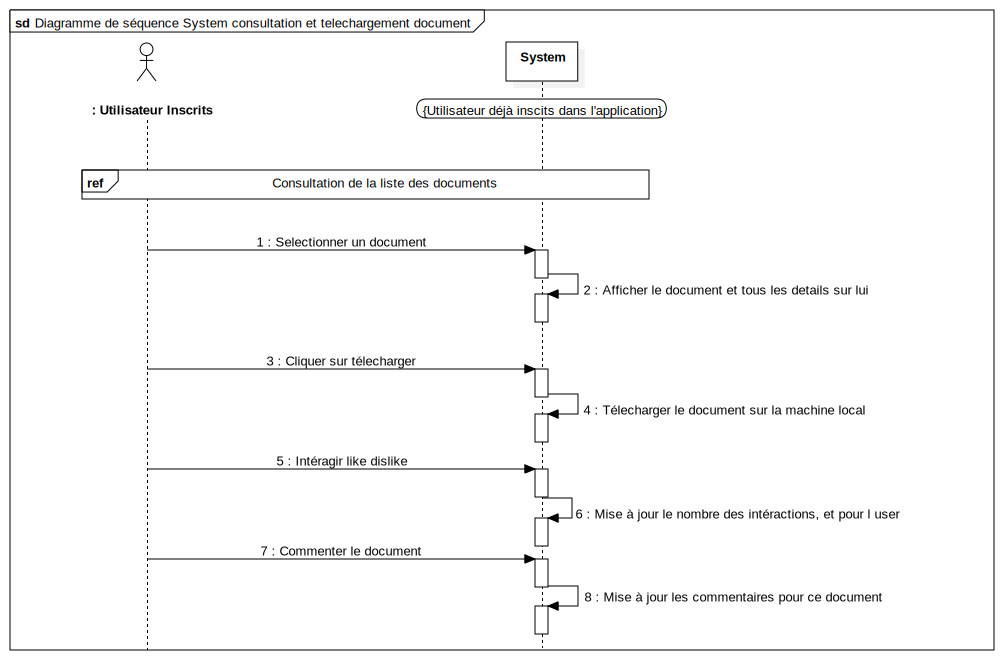
\includegraphics[width=1\textwidth]{Diagramme de séquence System consultation et telechargement document}
    \caption{Diagramme de séquence System consultation et telechargement document}
    \label{fig:mesh6}
\end{figure}

\newpage

\begin{figure}[h]
    \centering
    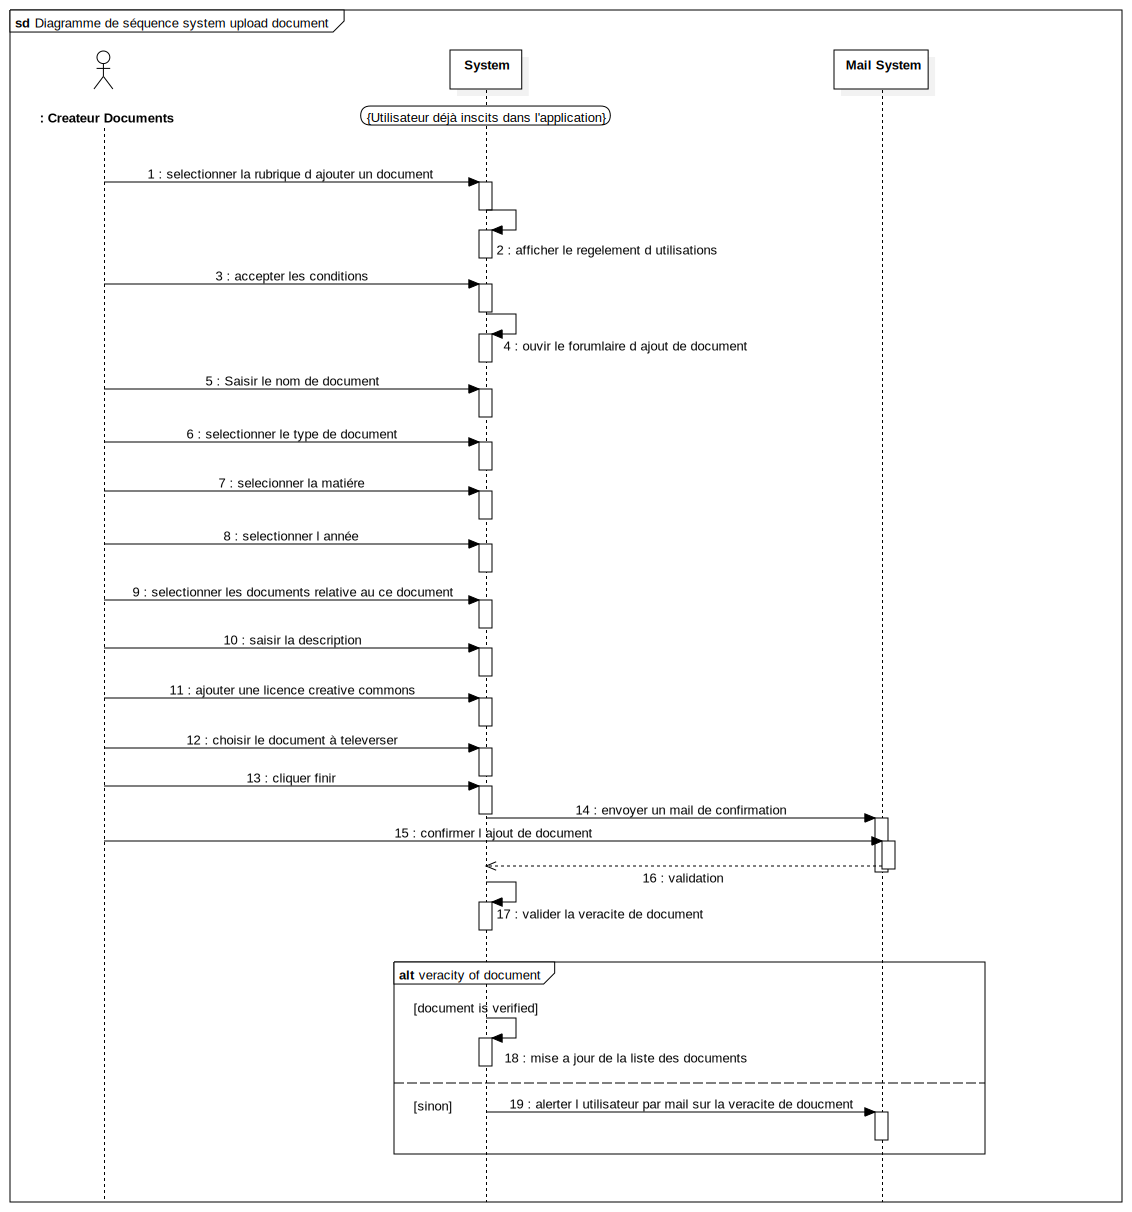
\includegraphics[width=.9\textwidth]{Diagramme de séquence system upload document}
    \caption{Diagramme de séquence system upload document}
    \label{fig:mesh6}
\end{figure}

\newpage

\begin{figure}[h]
    \centering
    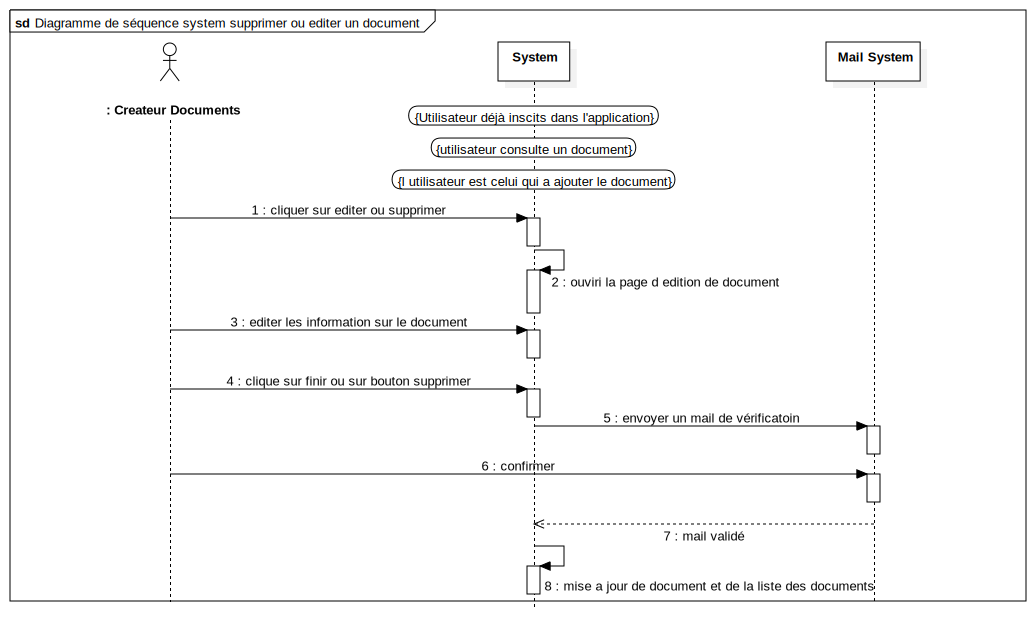
\includegraphics[width=1\textwidth]{Diagramme de séquence system supprimer ou editer un document}
    \caption{Diagramme de séquence system supprimer ou editer un document}
    \label{fig:mesh6}
\end{figure}

\newpage

\begin{figure}[h]
    \centering
    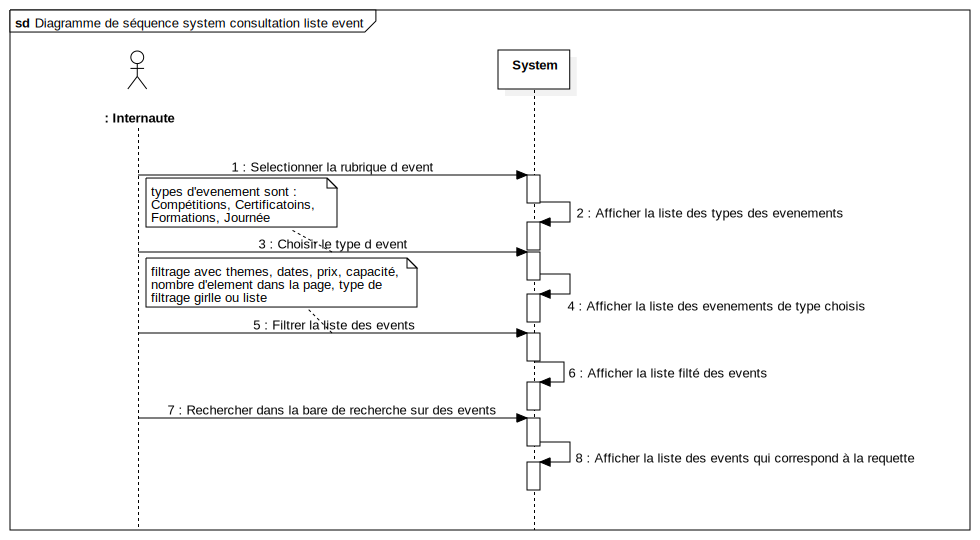
\includegraphics[width=1\textwidth]{Diagramme de séquence system consultation liste event}
    \caption{Diagramme de séquence system consultation liste event}
    \label{fig:mesh6}
\end{figure}

\newpage

\begin{figure}[h]
    \centering
    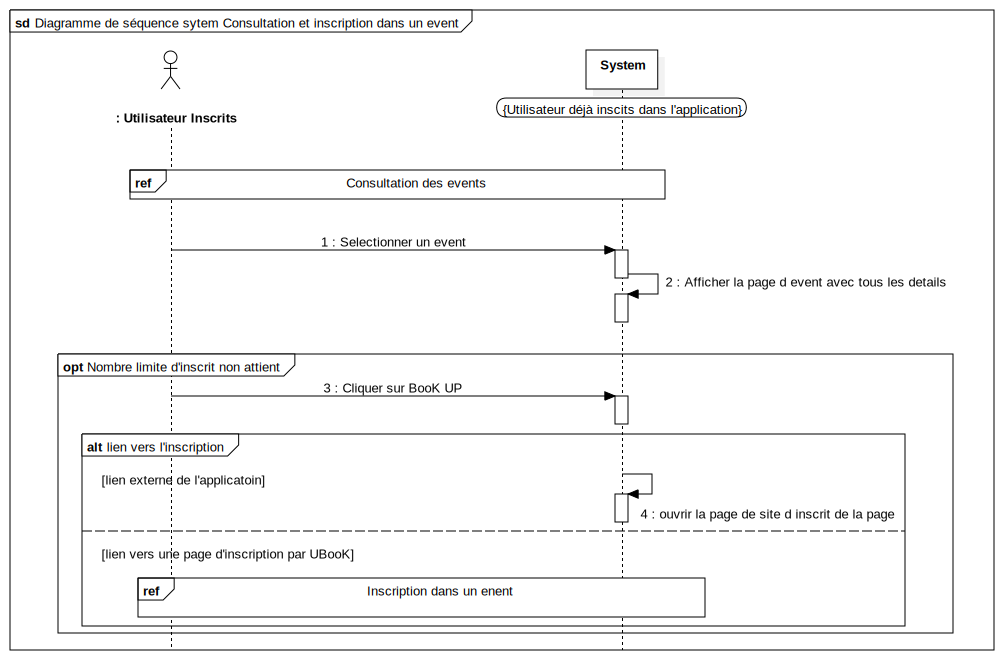
\includegraphics[width=1\textwidth]{Diagramme de séquence sytem Consultation et inscription dans un event}
    \caption{Diagramme de séquence sytem Consultation et inscription dans un event}
    \label{fig:mesh6}
\end{figure}

\newpage

\begin{figure}[h]
    \centering
    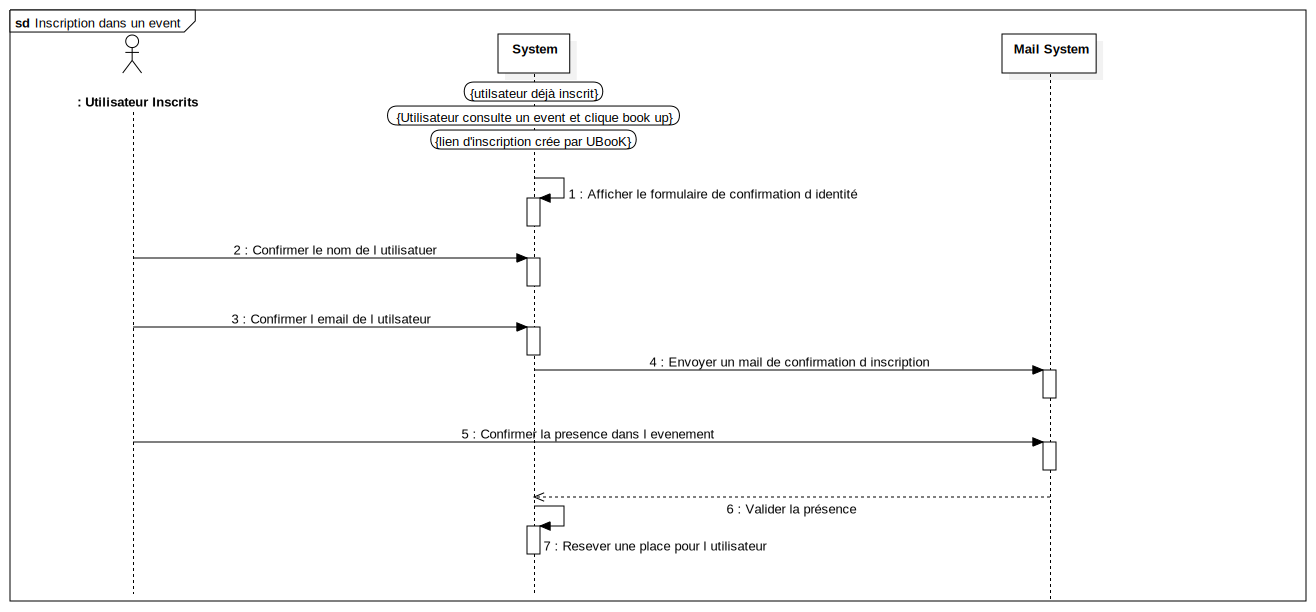
\includegraphics[width=1\textwidth]{Diagramme de séquence Inscription dans un event}
    \caption{Diagramme de séquence Inscription dans un event}
    \label{fig:mesh6}
\end{figure}

\newpage

\begin{figure}[h]
    \centering
    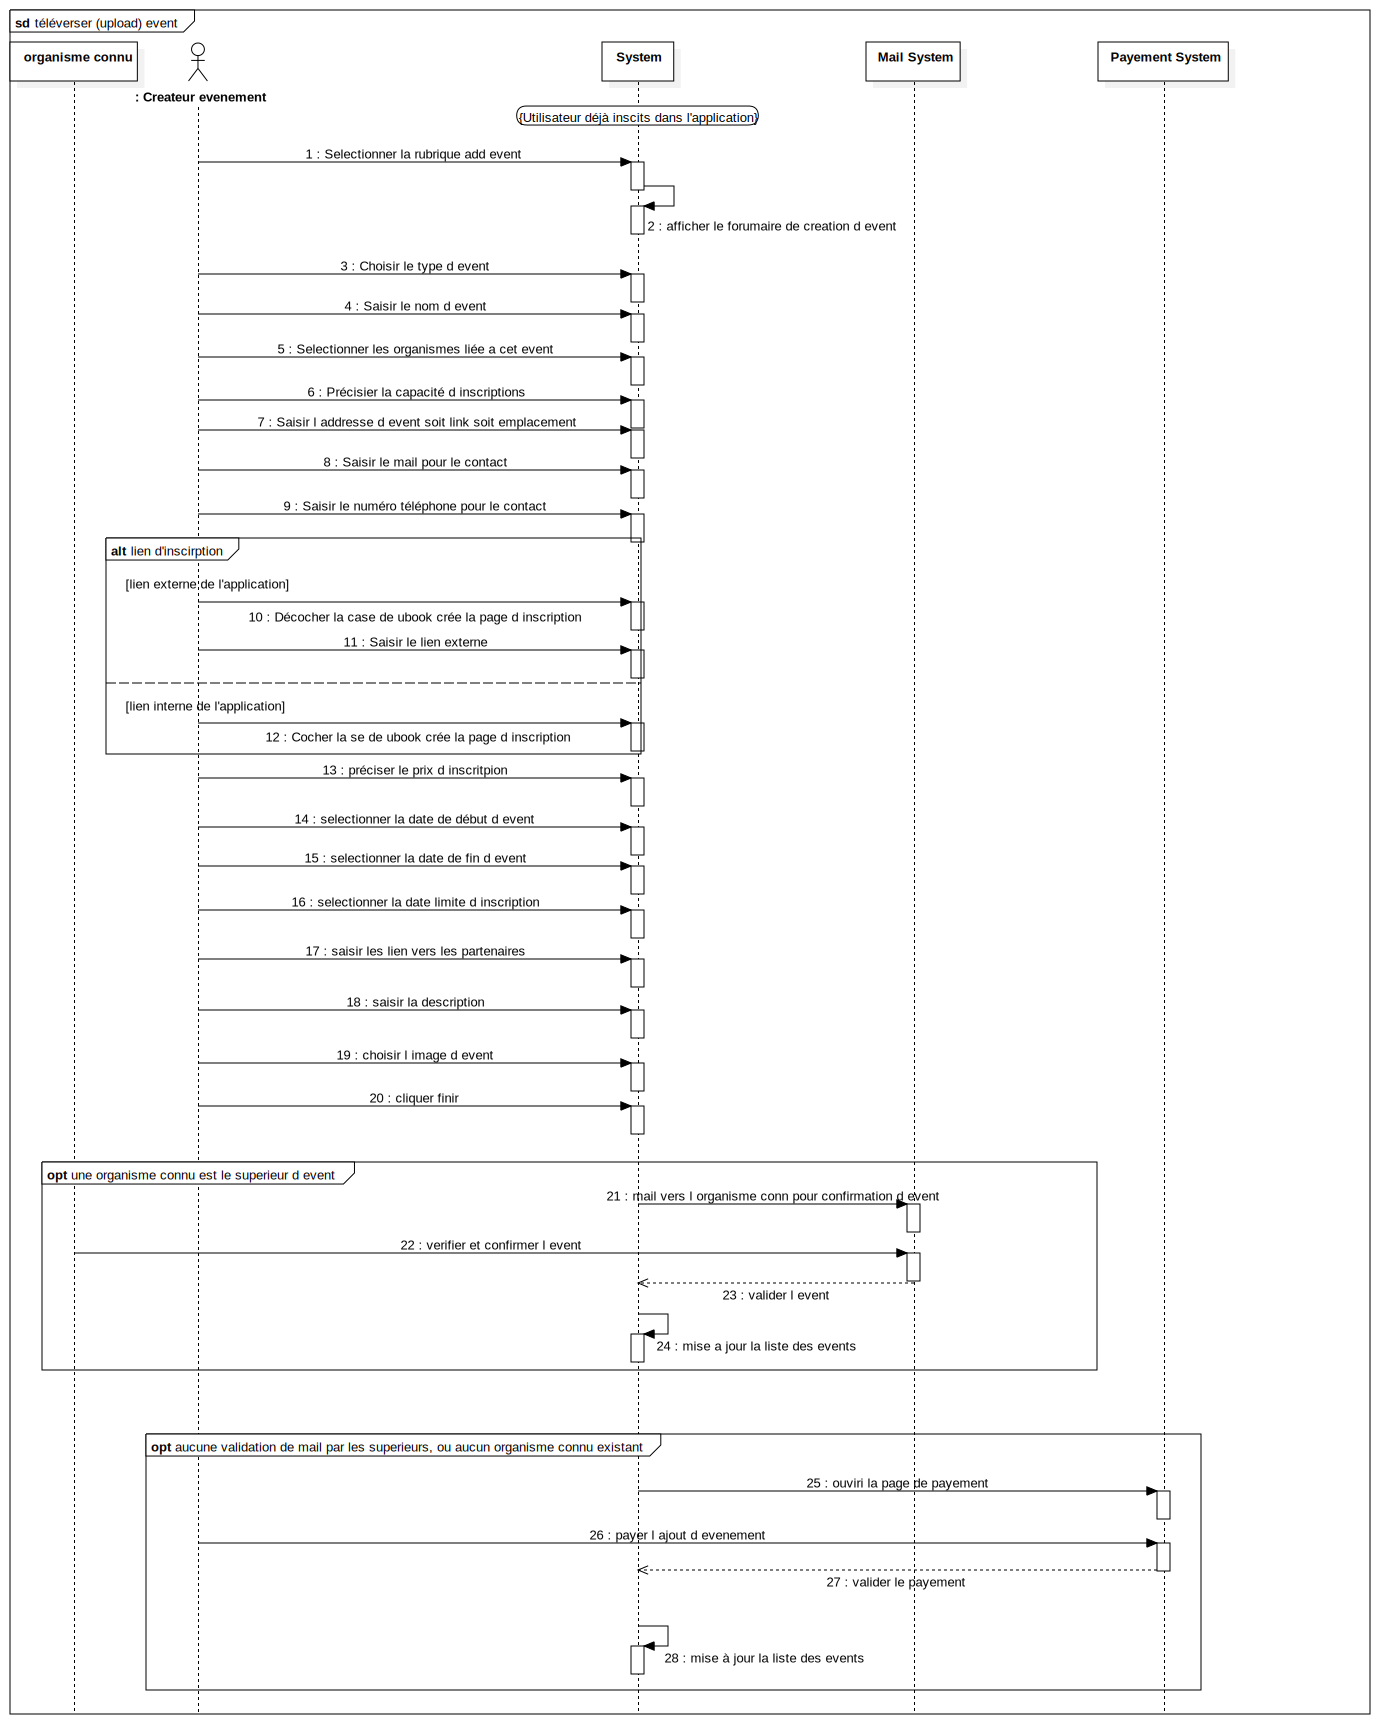
\includegraphics[width=.8\textwidth]{téléverser (upload) event}
    \caption{Diagramme de séquence Téléverser un event}
    \label{fig:mesh6}
\end{figure}

\newpage

\begin{figure}[h]
    \centering
    \includegraphics[width=1\textwidth]{eventEdit}
    \caption{Diagramme de séquence Editer un event}
    \label{fig:mesh6}
\end{figure}


\chapter{Conception et développement}

\section{Diagramme de classe analyse}

\begin{figure}[h]
    \centering
    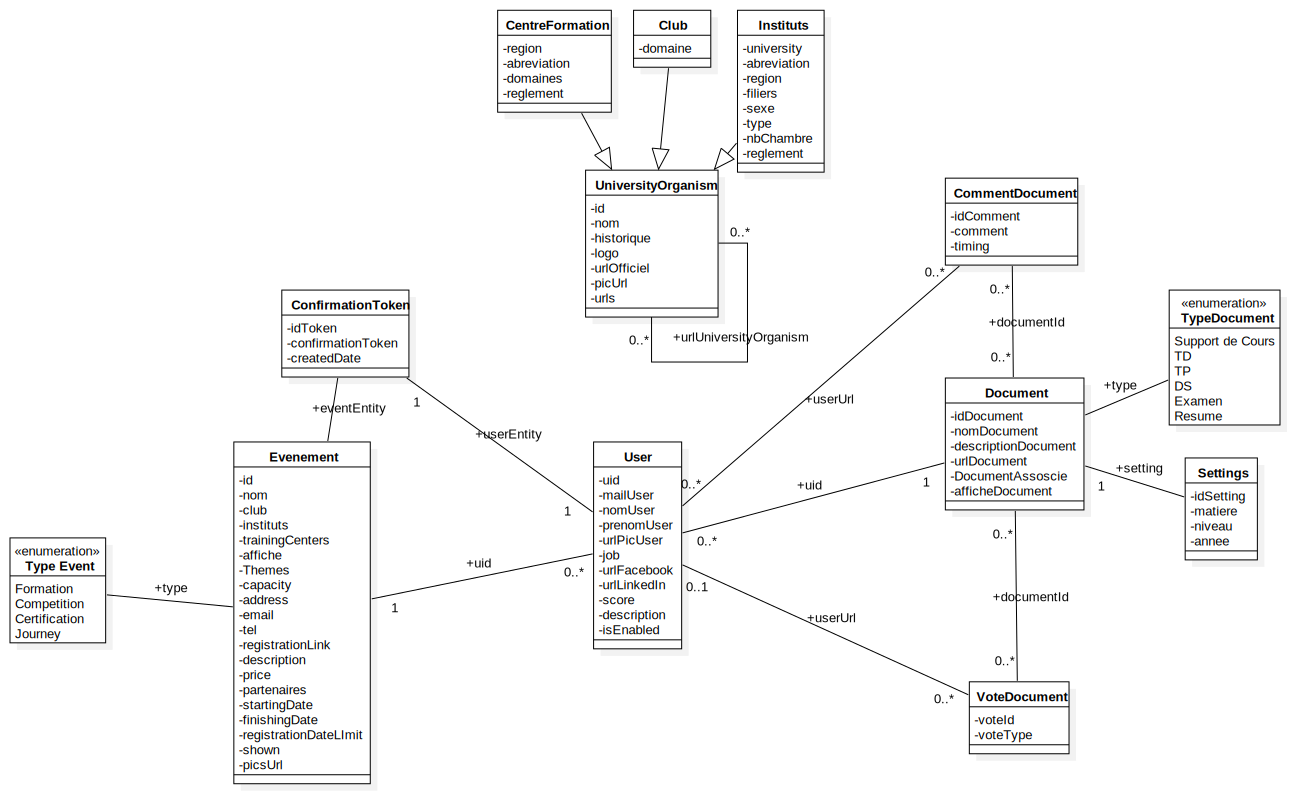
\includegraphics[width=1.2\textwidth]{AnalyseClassDiagram}
    \caption{Diagramme de classe d'Analyse}
    \label{fig:mesh6}
\end{figure}
\newpage


\section{Diagramme de classe conception}

\begin{figure}[h]
    \centering
    \includegraphics[width=1.2\textwidth]{Diagrammedeclasseconcpetion}
    \caption{Diagramme de classe d'Analyse}
    \label{fig:mesh6}
\end{figure}
\newpage

\section{Diagrammes de séquences objets}

\begin{figure}[h]
    \centering
    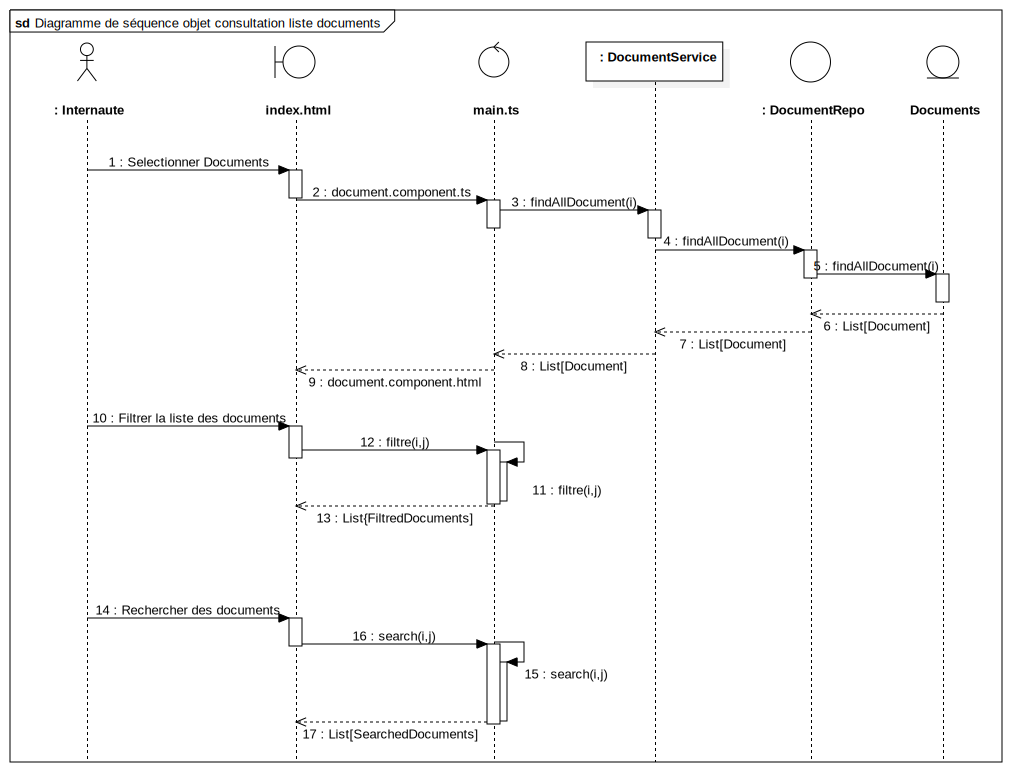
\includegraphics[width=1\textwidth]{Diagramme de séquence objet consultation liste documents}
    \caption{Diagramme de séquence objet consultation liste documents}
    \label{fig:mesh6}
\end{figure}
\newpage

\begin{figure}[h]
    \centering
    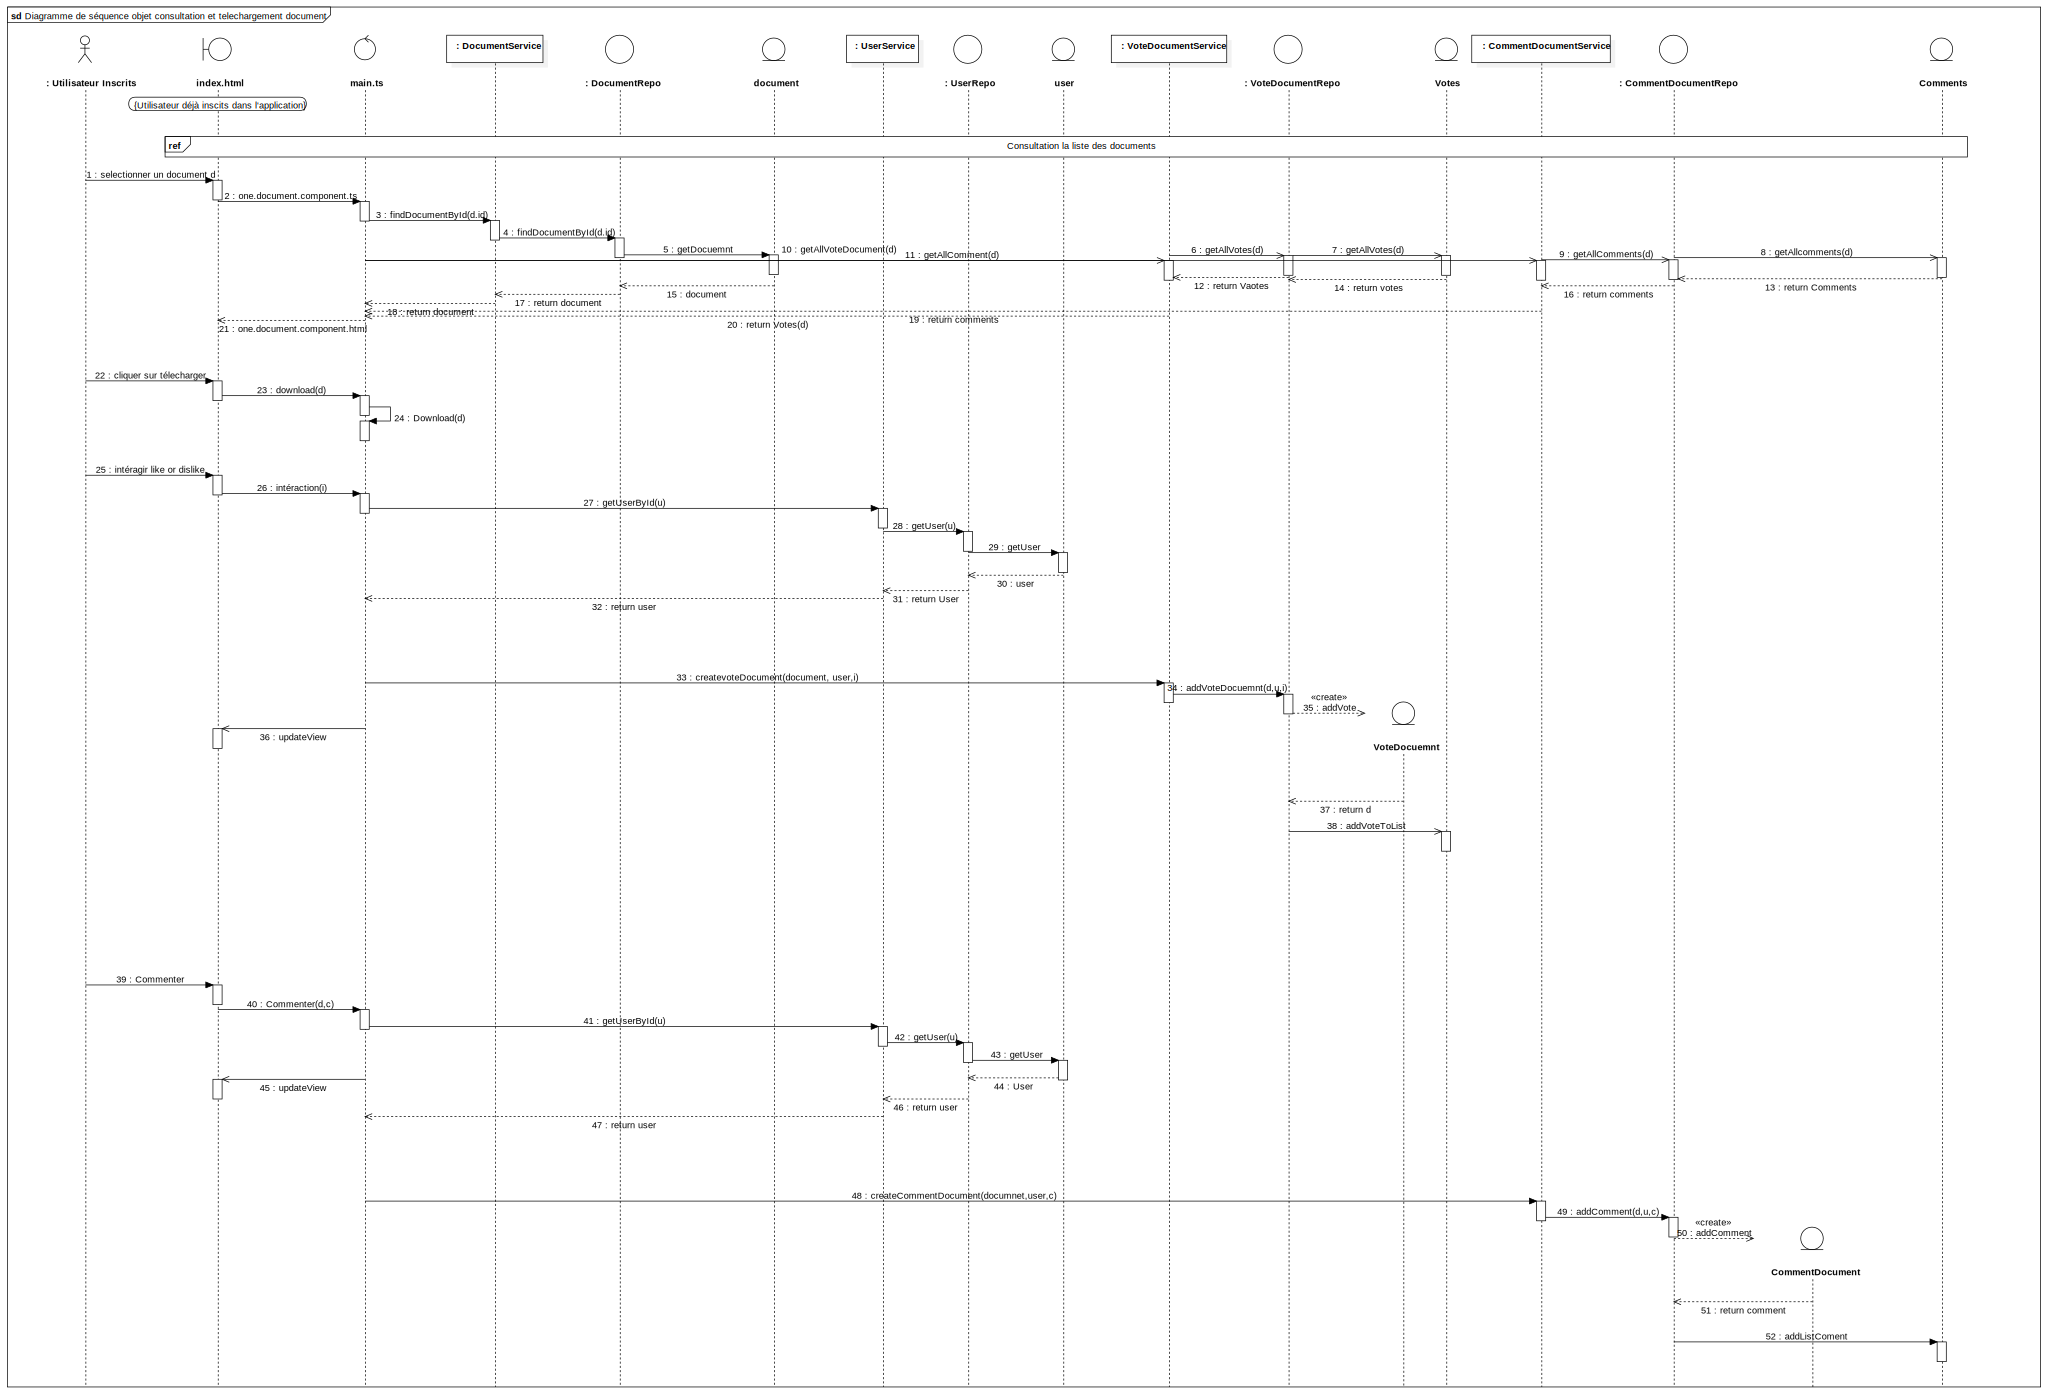
\includegraphics[width=1\textwidth]{Diagramme de séquence objet consultation et telechargement document}
    \caption{Diagramme de séquence objet consultation et telechargement document}
    \label{fig:mesh6}
\end{figure}
\newpage

\begin{figure}[h]
    \centering
    \includegraphics[width=1\textwidth]{Diagramme de séquence objet upload document}
    \caption{Diagramme de séquence objet upload document}
    \label{fig:mesh6}
\end{figure}
\newpage

\begin{figure}[h]
    \centering
    \includegraphics[width=1\textwidth]{DiagrammedeséquenceobjetConsultation listeevent}
    \caption{Diagramme de séquence objet  Consultation liste event}
    \label{fig:mesh6}
\end{figure}
\newpage

\begin{figure}[h]
    \centering
    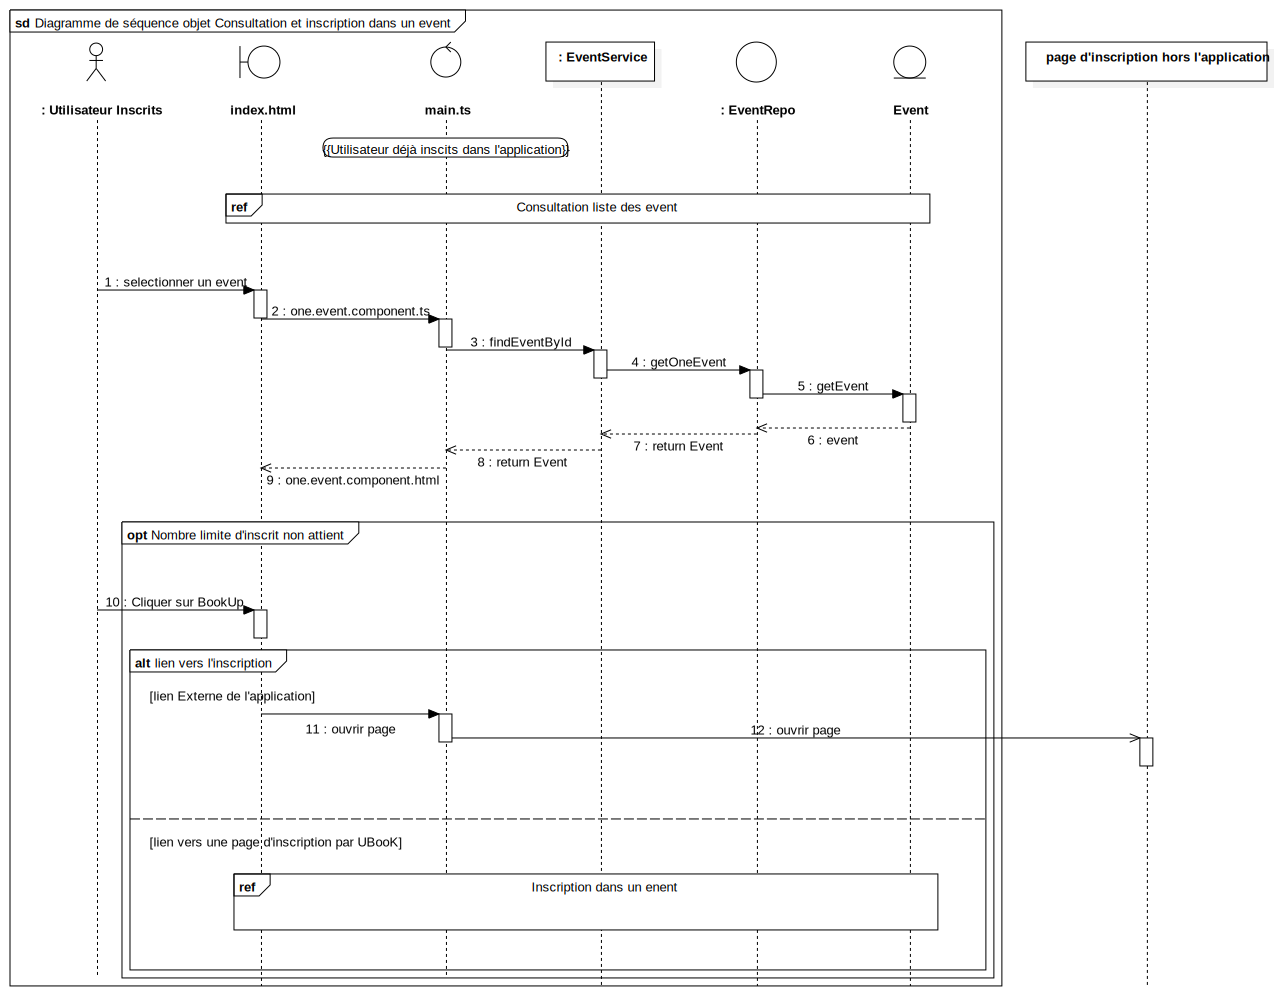
\includegraphics[width=1\textwidth]{Diagramme de séquence objet Consultation et inscription dans un event}
    \caption{Diagramme de séquence objet Consultation et inscription dans un event}
    \label{fig:mesh6}
\end{figure}
\newpage

\begin{figure}[h]
    \centering
    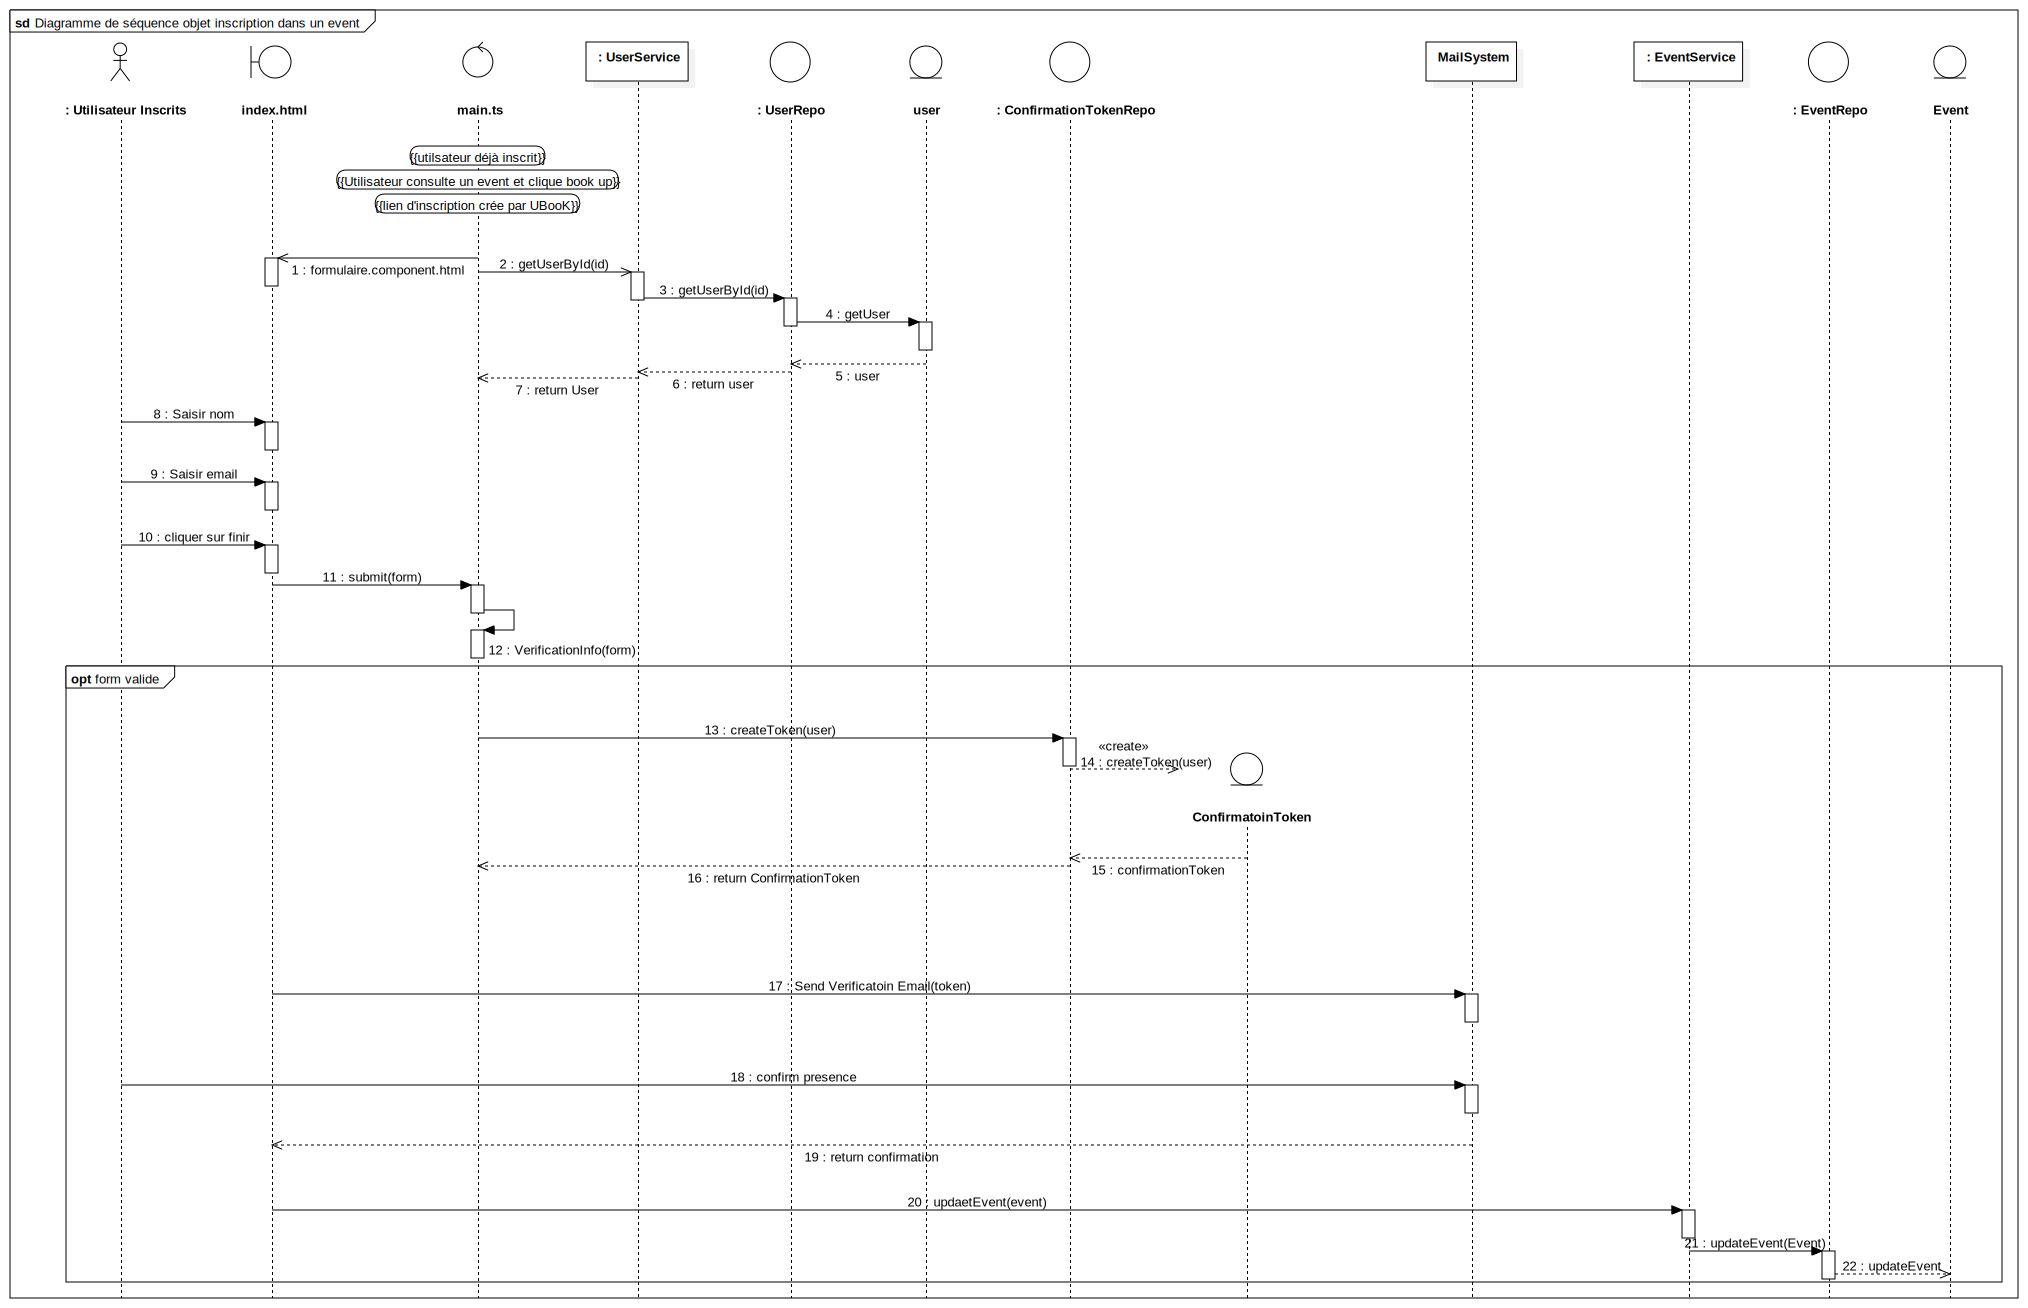
\includegraphics[width=1\textwidth]{Diagramme de séquence objet inscription dans un event}
    \caption{Diagramme de séquence objet inscription dans un event}
    \label{fig:mesh6}
\end{figure}
\newpage



\begin{figure}[h]
    \centering
    \includegraphics[width=1\textwidth]{Diagramme de séquence objet upload event }
    \caption{Diagramme de séquence objet upload event }
    \label{fig:mesh6}
\end{figure}
\newpage

\chapter*{Conclusion}
Dans cette partie nous avons bien exploré l'infrastructure de l'application UBooK qui traite l'aspect ethic la véracité d'information.\\
Dans la prochaine partie on étudie la partie recherche vers un modéle de véracité pour les document educatifs et pour les evenements universitaires.

\part{Vers un modéle de véracité}



\chapter{Etat de l'art}
\section*{Introduction}

UBooK est un réseau sociale qui offre des services 
de la vie estudiantine. Elle possède un espace de gestion 
d'événement et un espace de partage des documents éducatifs. 
\\Un des grands challenges c'est que le plateforme respecte 
les ethics et surtout la véracité d'information publié pour 
les documents éducatifs et les événements universitaires.
\\Alors dans ce chapitre on va Passer
 par les événements, on va les définir, 
enumérer les différent types et la politique 
fréquemment utilisé. 
\\Puis on s'intéresse sur les documents éducatives, on va différencier entre les types des documents éducatives et leurs métadonnées, Enfin citons une des politique pour les documents les licences Creative Commons 
\\Après on stop sur la véracité où on comprend mieux le
 concept et comment elle influence les documents et les 
événements et pour réaliser cet aspect on va raccourcir vers 
l'intelligence artificiel et elle même utilise l'indexation 
comme outil pour finir la tâche, ou on va se concentrer sur 
les deux derniers en les définir et mentionner les différentes
 types et modèles.
\section{Véracité}

\subsection{Notion de véracité}

Qualité morale de celui/celle qui ne trompe pas ou qui n'en a pas l'intention; en partic., qualité de celui/celle qui se garde de l'erreur et s'emploie à l'éviter dans ses paroles ou dans ses écrits. Synon. bonne foi*, exactitude, franchise, sincérité, véridicité.\\
Caractère de ce qui est conforme à la vérité, à la réalité. Synon. authenticité, exactitude.\\
Souci, recherche de l'exactitude, de la fidélité au réel, notamment dans la création artistique et littéraire.\\
VÉRACITÉ, (Morale.) la véracité ou vérité morale dont les honnêtes gens se piquent, est la conformité de nos discours avec nos pensées ; c’est une vertu opposée au mensonge.
\\(https://www.lalanguefrancaise.com/dictionnaire/definition/veracite)\\

La véracité fait référence à la provenance ou à la fiabilité de la source de données, à son contexte et à son importance pour l'analyse qui en découle. Des réponses à ces questions sont nécessaires pour déterminer la véracité de ces informations. La connaissance de la véracité des données nous aide à mieux comprendre les risques associés aux analyses et aux décisions commerciales basées sur cet ensemble de données particulier.

\subsection{La véracité en Big Data}

‘‘C'est l'un des enjeux majeurs de l'exploitation des Big Data. Faux profils
sur les réseaux sociaux, fautes d'orthographe, fraudes … Il est nécessaire
de multiplier les précautions (recoupement et enrichissement des données)
pour minimiser les biais liés au manque de fiabilité du Big Data.’’
\\(https://fr.wikipedia.org/wiki/veracite)\\

La véracité est le quatrième V du Big Data. Il s’agit de la qualité et de l’exactitude des données. Les données collectées peuvent comporter des éléments manquants, être inexactes ou ne pas fournir d’informations réelles et utiles. La véracité fait globalement référence au niveau de confiance dans les données collectées.

Les données peuvent parfois être confuses et difficiles à utiliser. Si elles sont incomplètes, . Un exemple tiré du domaine médical : si les données sur les médicaments que prend un patient sont incomplètes, la vie du patient peut être en danger.

La valeur et la véracité contribuent toutes deux à définir la qualité et les informations tirées des données. Dans un sens, c’est un facteur d’hygiène. En démontrant la véracité de vos données, vous montrez que vous avez porté un regard critique sur elles.

\subsection{La véracité pour les documents}

La véracité dans les documents se fait à travers la 
conformité des métadonnées avec le contenu du document, 
en plus un document vide ou bien qui mentionne une information 
fausse alors il n'est plus vrai.
Par exemple un document de grammaire 
française, ne doit pas être vide ou son contenu est 
autour de la musique. Si ces conditions sont validés alors ce 
document est vrai. 
Aussi que la véracité est lié d'authenticité si l'auteur 
n'est pas celui le propriétaire de document alors aucune 
véracité existante.
\subsection{La véracité pour les evenements}

La véracité pour les événements signifie que la certitude de 
déroulement de cet événement, en plus qu'il est bien conforme 
aux thématiques mentionnées. \\Mais la véracité ne se limite pas au
 événement lui même mais aussi les inscription aux evénement 
doit être vrai car on peut y avoir des faux inscritption pour 
les participants.

\section{Indexation}

\subsection{Notion d'indexation}

L'indexation automatique de documents est un domaine de l'informatique et des sciences de l'information et des bibliothèques qui utilise des méthodes logicielles pour organiser un ensemble de documents et faciliter ultérieurement la recherche de contenu dans cette collection.La multiplicité des types de documents (textuels, audiovisuels, Web) donne lieu à des approches très différentes, notamment en termes de représentation des données. Elles reposent néanmoins sur un socle de théories communes, telles que l'extraction de caractéristiques, le partionnement de données (ou clustering), la quantification, et plus généralement la recherche d'information.
\\(https://fr.wikipedia.org/wiki/Indexation\_automatique\_de\_documents)\\

En général, l'indexation fait référence à l'organisation des données selon un schéma ou un plan spécifique. En informatique, le terme a diverses utilisations similaires, notamment pour rendre les informations plus présentables et accessibles.
\\(https://fr.theastrologypage.com/indexing)\\

L'indexation des documents consiste à associer des mots clés et informations à chaque documents en fonction du plan de classement, afin de faciliter, ensuite, la recherche, l’accès et le traitement par les utilisateurs.

Alors l’indexation est un ensemble des méthodes et techniques pour l’acquisition, l’organisation, le stockage, la recherche et la sélection d’information pertinente pour un utilisateur


\subsection{Modéles de recherche d'information}

Le modéle de recherche d'information RI comprend la fonction de décision fondamentale qui permet
d’associer à une requête, l’ensemble des documents pertinents
à restituer.Il est étroitement lié au modèle de représentation des
documents et requêtes.\\
L’appariement requête-documents consiste à calculer un score,
supposé représenter la pertinence du document vis-à-vis de la
requête.\\
Ce score est souvent calculé à partir d’une fonction ou une
probabilité de similarité, en fonction du modèle utilisé, qui tient
compte du poids des termes dans les documents.
L’assignation d’un score de pertinence à un document permet
d’ordonner les documents renvoyés à l’utilisateur

\begin{figure}[h]
    \centering
    \includegraphics[width=1\textwidth]{indexation}
    \caption{Classification des modèles selon la théorie}
    \label{fig:mesh2}
\end{figure}

\begin{itemize}
\item Modéle Booléen : C’est le premier modèle de RI,
Introduit en 1983 par Salton et McGill, 1 er SRI commercial pour 3 décennies (60-90), Basé sur la théorie des ensembles et l’algèbre de Boole, L’interface d’interrogation de la plupart des moteurs de
recherche est basée sur les principes de ce modèle.\\
Il considère que les termes de l’index sont présents ou
absents d’un document\\
Les poids des termes dans l’index sont binaires : w i,j = \{0, 1\}\\
Un document est soit pertinent soit non pertinent pour une
requête donnée : Pertinence binaire, et jamais partielle.

\item Modéle Booléen Pondéré : Extension du modèle booléen en intégrant des
pondérations (dénotant la représentativité d’un terme
pour un document) \\
Fonction de correspondance non binaire (on se passe des
implications logiques) basée sur une similarité notée Sim

\item Modéle vectoriel : Dans des très grandes collections de documents, le
résultat de recherche pour une requête donnée dépasse
généralement la capacité des utilisateurs à examiner tous
les documents de l’ensemble retourné\\ Affecter un score (degré de similarité), à chaque document
relativement à une requête donnée : le document le plus
pertinent devrait avoir le score le plus élevé.
\item ...
\end{itemize}
\section{IA et ML}

\subsection{Notion d'Intéligence Artificiel}

L'intelligence artificielle (IA, ou AI en anglais pour Artificial Intelligence) consiste à mettre en œuvre un certain nombre de techniques visant à permettre aux machines d'imiter une forme d'intelligence réelle. L'IA se retrouve implémentée dans un nombre grandissant de domaines d'application.\\
Les domaines d'application de l'intelligence artificielle sont nombreux. Elle est présente dans les appareils photo des smartphones. En mode nocturne, elle permet d'adapter la colorimétrie à l'environnement, et de redonner à une façade éclairée son éclat originel pour le reproduire fidèlement sur votre cliché.
\\(https://www.futura-sciences.com/tech/definitions/informatique-intelligence-artificielle-555/)

En termes simples, l'intelligence artificielle (IA) fait référence à des systèmes ou des machines qui imitent l'intelligence humaine pour effectuer des tâches et qui peuvent s'améliorer en fonction des informations collectées grâce à l'itération.\\
(https://www.oracle.com/fr/artificial-intelligence/what-is-ai/)\\

Il y'a qutare écoles en IA : 
\begin{itemize}
\item Penser comme des humains : Les efforts passionnats pour pousser les ordinateurs à penser d'en fabriquer des machines avec cerveaux au sens le plus latéral.(Haugeland, 1985)
\item Penser Rationnellement : L'etude des facultés mentales par l'élaboration des modéles mathématiques.(Charniak et McDermott, 1987)
\item Agir comme des humains : L'etude des moyens qui permettent aux ordinateurs de faire des choses qui pour le moment sont mieux faites par des hommes.(Rich et Knight, 1991)
\item Agir rationnellement : L'etude et la conception d'agents intelligents.(Poole, 1998)
\end{itemize}

\subsection{Notion d'Apprentissage Automatique}

L'apprentissage automatique est une branche de l'intelligence artificielle
(IA) et de l'informatique qui utilise principalement des données et des
algorithmes pour imiter la manière dont les être humains apprennent, en
améliorant progressivement sa précision.
L'apprentissage automatique est une composante importante du domaine
en pleine expansion qu'est la science des données. Grâce à l'utilisation de
méthodes statistiques, des algorithmes sont entraînés à effectuer des
classifications ou des prévisions, ce qui permet de découvrir des
informations essentielles dans le cadre de projets d'exploration des
données. Ces informations permettent ensuite de prendre des décisions
dans les applications et les entreprises, et ont idéalement un impact sur les
principales métriques de croissance. Au fur et à mesure que le big data
poursuit son développement et sa croissance, les besoins en spécialistes
des données va augmenter, ce qui les obligera à contribuer à l'identification
des questions commerciales les plus pertinentes et, par conséquent, des
données permettant d'y répondre.\\
(https://www.ibm.com/cloud/learn/machine-learning)


En machine learning il y’en a deux branches, l’apprentissage supervisé et non supervisé.
Ce dernier consiste à prédire par oui ou non (Vrai ou Faux) à une proposition ‘statement’ après un entraînement sur deux clusters. Son rôle est la plupart de différencier entre deux groupes. Les fameux modèles sont K-Means, CAH...
Et l’apprentissage supervisé lui même a deux sous branches le classification et la régression.
Pour le classification son but est de classifier et donner une famille ou un valeur brute pour une donnée, la plupart d’utilisation de classification et de prédire un type de donnée. Les fameux modèles sont : KNN, CNN,Arbre de décision…
Mais pour la régression et de donner un intervalle de valeur pour une donnée, la plupart d’utilisation de régression est dans la prédiction des valeur numérique, ou prédiction des pourcentages. Les fameux modèles sont : Linear Régression, Polynomial Regression...
\subsection{IA Et Evenements}

\subsubsection{Web Scrapping}
Le web scraping (parfois appelé harvesting) est une technique
d'extraction du contenu de sites Web, via un script ou un programme, dans
le but de le transformer pour permettre son utilisation dans un autre
contexte, par exemple le référencement\\
(https://fr.wikipedia.org/wiki/WebScrapping)\\
le grattage du web permet de chercher un ensemble 
d’information sur des
sites bien spécifiques, c’est modèle d’IA qui parcours 
le web sémantique et
vérifie les balises HTML.
Les meilleurs bibliothèques dans le web scraping sont :
Scrapy (Python), BeautifulSoup (Python), Requests (Python), LXML
(Python), Selenium (Python), Jsoup (JAVA) ...

Le grattage du web permet de récupérer les vraies événements 
en cherchant dans les sites et les pages d'événement 
confiants

\subsection{Les modéles ML qui traitent la véracité des documents}

Les fameux modèles qui traitent la véracité des document utilisent le traitement automatique de langage naturel TAN :\\ Le traitement automatique du langage naturel imite la compréhension
humaine des mots et des phrases et permet maintenant aux modèles
d'apprentissage automatique de traiter de grandes quantités d'informations
avant de fournir des réponses précises aux questions qui leur sont posées.
L'utilisation du TAN permet de comprendre le contenu du document et vérifier sa véracité.
\\Autre modèles qui traitent la véracité sont la classification des documents par l'apprentissage automatique, on mentionne en titre d'exemple KNN, Arbre de décision, Naive Bayes
Dans la section suivante on suit les travaux anciens et leurs modèles qui traitent la véracité des documents.

\section{Travaux anicennes}

\subsection{Feuille de route}

Dans cette partie on va s’intéréssé sur les travaux anciens qui est autours la véracité. 
En premier lieu on étudie les modéles sur la véracité d’information de facon générale
En second lieu on étudie les modéles sur la véracité principalement des documents

\subsection*{Véracité des information de facon générale}

\subsection{Système d’aide à la décision pour la véracité des données dans le contexte de Big Data}

Comme la fiabilité des données est un challenge concrétisé par la
dimension de véracité dans le contexte de Big Data, et afin d’extraire des
données fiables à partir des systèmes d’information ou les données peuvent
incomplète, imprécisé, vague,…etc. Ce travail répond à l’objectif de la
création d’un système basé sur la théorie de Rough sets* de véracité de
données dans un contexte de Big data.
\\
*La théorie des ensembles approximatifs (RST) est une approximation
formelle de la théorie des ensembles conventionnelle qui prend en charge
les approximations dans la prise de décision. Cette approche peut extraire
des connaissances d'un domaine problématique de manière concise et
conserver le contenu de l'information tout en réduisant la quantité de
données impliquée.\\ \\
Url: https://www.academia.edu/42880013/Syst\%C3\%A8me\_daide\_\%C3\%A0\_la\\\_d\%C3\%A9cision\_pour\_la\_v\%C3\%A9racit\%C3\%A9\_des\_donn\%C3\%A9es\_dans\_le\\\_contexte\_de\_Big\_Data)


\subsection{Modèle probabiliste avec support mutuel des valeurs similaires}

Basé sur l’analyse bayésienne, TruthFinder (Yin et al., 2008) calcule la
fiabilité de l’information donnée par une source. Il s’appuie sur l’honnêteté
de la source d’information et suit l’heuristique selon laquelle si les valeurs
fournies sont essentiellement vraies pour de nombreux cas, alors elles
seront aussi probablement vraies pour d’autres cas. Mais dans notre cas ce n’est plus fonctionnel car on cherche à un modèle ou le source est unique.
Et l’information vient d’un seul source, ne peut par étre des sources
différents, en respectant la non redondance.
\\ \\(Yin, X., Han, J., and Yu, P. Truth discovery with multiple conflicting
information providers on the web. Knowledge and Data Engineering,
IEEE Transactions on, 20 :796 – 808, 07 2008. doi :
10.1109/TKDE.2007.190745.)

\subsection{Découverte de la vérité par corroboration d’informations}

C’est un ensemble de trois algorithmes proposés dans (Galland et al.,
2010) : COSINE, 2 ESTIMATES et 3-ESTIMATES. COSINE initialise la
fiabilité de chaque valeur et de chaque source. Il calcule de façon itérative
la fiabilité d’une source comme une fonction linéaire de sa fiabilité
précédenteMais dans notre cas ce n’est plus fonctionnel car on cherche à
un modèle ou le source est unique. Et l’information vient d’un seul source,
ne peut par étre des sources différents, en respectant la non redondance.
\\ \\(Galland, A., Abiteboul, S., Marian, A., and Senellart, P. Corroborating
information from disa- greeing views. In Proceedings of the third ACM
international conference on Web search and data mining, pages 131–140,
2010.)

\subsection{Modèle de vérité latente}

Ce modèle utilise les réseaux bayésiens pour estimer la fiabilité de
l’information. " Latent Truth Model " (LTM) est proposé dans (Zhao et al.,
2012). Il se base sur deux hypothèses :
\\— les données doivent contenir un seul attribut avec une valeur atomique ;
\\— la gestion de plusieurs valeurs vraies pour le même attribut.
Pour chaque source, LTM considère les probabilités à priori pour qu’elle
soit un vrai positif ou un faux positif avec des erreurs négatives. Enfin, les
valeurs dont le degré de fiabilité est supérieur à 0.5 sont considérées
comme vraies. Il faut noter que le LTM peut ne pas détecter des valeurs
vraies pour certains attributs.\\ \\(Zhao, B., Rubinstein, B. I., Gemmell, J., and Han, J. A bayesian approach
to discovering truth from conflicting sources for data integration. arXiv
preprint arXiv :1203.0058, 2012.)

\subsection{Découverte de la vérité par estimation de la vraisemblancemaximale}

Basée sur la maximisation de la vraisemblance pour quantifier la fiabilité
des sources et la justesse des valeurs, " Maximum Likelihood Estimation "
(MLE) est proposé dans (Wang et al., 2012). MLE traite seulement les
observations booléennes positives et ignorent celles négatives. Dans son
algorithme, MLE initialise les paramètres des sources :
\\— a(s) probabilité pour que la source s signale une valeur vraie et elle est
effectivement vraie
\\— b(s) probabilité pour que la source s signale une valeur vraie alors
qu’elle est en réalité fausse.
De façon itérative, MLE calcule la probabilité conditionnelle d’une valeur
v d’être vraie sur la base des probabilités (a(s), b(s)) de sa source et celle
des sources ne fournissant pas la valeur v. Ensuite la confidence de chaque
valeur est calculée itérativement. Après cela, MLE procède à la mise à jour
des probabilités (a(s), b(s)) de chaque source. Les itérations s’arrêtent à la
convergence de a(s) et b(s). Une importante observation faite dans les
expériences de l’article (Waguih and Berti-Equille, 2014) permet de dire
que MLE ne peut pas être utilisé avec de grands nombre de sources
(>5000).
Mais dans notre cas ce n’est plus fonctionnel car on cherche à un modèle
ou le source est unique. Et l’information vient d’un seul source, ne peut
par étre des sources différents, en respectant la non redondance.
\\ \\(Wang, D., Kaplan, L., Le, H., and Abdelzaher, T. On truth discovery in
social sensing : A maximum likelihood estimation approach. IPSN’12 -
Proceedings of the 11th International Conference on Information
Processing in Sensor Networks, 04 2012. doi :10.1145/2185677.2185737.)

\subsection{Découverte de la vérité avec dépendance de sources par copie}

Ici, nous parlerons des algorithmes de recherche de vérité qui tiennent
compte de la relation qui existe entre sources. DEPEN est le premier
proposé dans (Dong et al., 2009). C’est un modèle bayésien de recherchede vérité qui prend en considération les relations de copie qui peuvent
exister entre les sources en pénalisant le vote d’une source si elle est
détectée comme étant la copie d’une autre source. Le calcul de la matrice
de dépendance entre les sources est très coûteux surtout lorsque les
données en entrée sont volumineuses ; c’est un des goulots d’étranglement
majeurs de DEPEN et ses extensions.
\\ \\(Dong, X., Berti-Equille, L., and Srivastava, D. Integrating conflicting data
: The role of source dependence. PVLDB, 2 :550–561, 08 2009.)

\subsection{Analyse de crédibilité latente}

LCA (" Latent Credibility Analysis ") est un modèle probabiliste proposé
dans (Pasternack and Roth, 2013). Il utilise aussi l’algorithme de
maximisation de la vraisemblance pour calculer la probabilité des valeurs
en regroupant les mêmes attributs d’un même objet en une même donnée
dans un ensemble d’exclusion mutuelle où il n’existe qu’un seul élément
vrai. LCA est une approche flexible et puissante pour modéliser le
problème de la crédibilité de l’information.
\\ \\(Pasternack, J. and Roth, D. Latent credibility analysis. In Proceedings of
the 22nd international conference on World Wide Web, pages 1009–1020,
2013.)

\subsection{Découverte de la vérité dans plusieurs domaines de sources contradictoires ayant des vérités multiples}

Ce modèle est un modèle probabiliste et bayésien à la fois, qui intègre le
score d’expertise de domaine et le score de confiance pour la
détermination de la vérité. DART (Domain AwaRe Truth Discovery) est un
modèle proposé dans (Lin and Chen, 2018). L’idée de base est la
construction d’un modèle, qui contient deux composantes intégrales : la
modélisation de l’expertise du domaine concernant la richesse des
données, et la modélisation de l’agrégation de la vérité à partir des
réponses de chaque source.
\\ \\(Lin, X. and Chen, L. Domain-aware multi-truth discovery from
conflicting sources. Proceedings of the VLDB Endowment, 11(5) :635647,
2018.)

\subsection{Découverte de la vérité avec partitionnement des attributs}

Proposée dans (Lamine Ba et al., 2015), c’est une méthode de recherche de
vérité qui se base sur le partitionnement des attributs des objets. Son
objectif est donc d’estimer une partition optimale de l’ensemble des
attributs de telle sorte qu’en appliquant indépendamment n’importe quel
algorithme de recherche de vérité de référence sur chaque sous ensemble
de la partition, on maximisera la précision de cet algorithme. L’estimation
de la partition optimale dans ce cas se base seulement sur la qualité de
l’algorithme de recherche.
\\ \\(Lamine Ba, M., Horincar, R., Senellart, P., and Wu, H. Truth finding with
attribute partitioning. In Proceedings of the 18th International Workshop
on Web and Databases, WebDB’15,page 27–33, New York, NY, USA,
2015. Association for Computing Machinery. ISBN 9781450336277. doi :
10.1145/2767109.2767118. URL https://doi.org/10.1145/2767109.2767118
.)

\subsection{Modèle probabiliste pour la découverte de la vérité avec des corrélations d’objets avec des contraintes}

Ce modèle probabiliste se base sur la corrélation entre les objets en tenant
compte de certaines contraintes qui lui sont fournies en entrée. "
Constrained Truth Discovery " (CTD) est proposé dans (Yang et al., 2019)
et formulé comme un problème d’optimisation sous contraintes. Le
processus de découverte de la vérité intègre les contraintes de type "
Denial Constraints (DCs) " (Chomicki and Marcinkowski, 2005) à l’aide
d’un formalisme basé sur la logique du premier ordre universellement
quantifié qui peut exprimer un grand nombre de relations effectives et
largement existantes entre les objets. Sur cette base les auteurs proposent
des algorithmes pour partitionner les objets en groupes disjoints en
générant des contraintes arithmétiques pour chaque groupe disjoint
séparément. Ensuite, les vraies valeurs des attributs des objets dans chaque
groupe disjoint sont dérivées en minimisant une fonction objective sous les
contraintes arithmétiques correspondantes.
\\ \\(Yang, Y., Bai, Q., and Liu, Q. A probabilistic model for truth discovery
with object correlations. Knowledge-Based Systems, 165 :360–373, 2019.)
\\ \\(Chomicki, J. and Marcinkowski, J. Minimal-change integrity maintenance
using tuple deletions.Information and Computation, 197(1-2) :90–121,
2005.)
\subsection{Vérification de faits par partitionnement de données}

Dans ce travail, nous intéresse la vérification de faits dans un domaine où
les données ont une structure inhérente qui n’est pas connue à l’avance.
Pour résoudre ce problème il a été conçu et proposé un algorithme, appelé
TD-AC, de partitionnement de données intelligent basé sur la méthode de
clustering des données des k-moyennes du domaine de l’apprentissage
automatique. Pour choisir la partition optimale, l’indice de silhouette a été
choisis. Ensuite, (OSIAS NOËL) a proposé une validation des
performances de l’algorithme. Pour ce faire, il l’a comparé à l’approche
proposée dans (Lamine Ba et al., 2015) et aux algorithmes de découverte
de la vérité standards sur des jeux de données synthétiques, semi
synthétiques et réelles. Enfin, (OSIAS NOËL) a montré que TD-AC a une
complexité en temps comparable à celle des algorithmes standards
contrairement à l’algorithme brute force dans (Lamine Ba et al., 2015).
Cependant, nous avons observé que lorsque le jeu de données est
caractérisé par beaucoup de valeurs, cet approche est moins
performante : ceci à cause de l’utilisation d’une matrice creuse comme
entrée de l’algorithme de clustering entraînant une difficulté à trouver la
partition optimale.
\\ \\(URL : OSIAS NOËL NICODÈME FINAGNON TOSSOU 3 Mars 2021Url
https://www.researchgate.net/publication/349733401\_Verification\_de\_faits \_par\\\_partitionnement\_de\_donnees\_Truth\_discovery\_by\_data\_partitioning)

\subsection*{Véracité des documents}

\subsection{Incorporation de phrases (SIF)}

Les travaux qui ont combinaient l'incorporation de mots en utilisant des
opérations sur des vecteurs et des matrices pour dériver l'incorporation de
phrases ou de phrases. Les résultats ont montré que l'exploitation des
vecteurs par multiplication par coordonnées permet d'obtenir de très
bonnes performances dans les opérations binaires étudiées. Et concentré
sur les représentations distribuées des phrases. Ils nécessitaientgénéralement une analyse syntaxique et il a été démontré que le résultat
fonctionnait pour les représentations au niveau de la phrase. Une autre
approche a mis en place un algorithme non supervisé pour apprendre les
représentations distribuées de phrases ou de documents. Leurs expériences
ont indiqué que leur méthode était compétitive avec les méthodes de
pointe.
\\ \\(Song, M., Zhao, X., Liu, Y., Zhao, Z.: Text sentiment analysis based on
convolutional neural network and bidirectional LSTM model. In: Zhou,
Q., Miao, Q., Wang, H., Xie, W., Wang, Y., Lu, Z. (eds.) ICPCSEE 2018.
CCIS, vol. 902, pp. 55–68. Springer, Singapore (2018).
https://doi.org/10.1007/978-981-13-2206-8 6 )

\subsection{Analyse syntaxique}

L'analyse syntaxique est l'une des technologies de base du traitement du
langage naturel et la pierre angulaire d'une compréhension approfondie du
langage. La tâche de l'analyse syntaxique est d'identifier les composants
syntaxiques contenus dans la phrase et la relation entre ces composants, en
utilisant généralement des arbres d'analyse pour représenter les résultats de
l'analyse syntaxique.
\\ \\(Wu, W., Zhou, J., Qu, W.: A survey of syntactic parsing based on
statistical learning. J.Chin. Inf. Process. 27(3), 9–19 (2013) )

\subsection{Calcul de l'incorporation de phrases en fusionnant l'arbre d'analyse syntaxique et l'incorporation de mots}

L'article propose une méthode d'incorporation de phrases basée sur les
résultats de l'arbre d'analyse syntaxique et des vecteurs de mots. L'ordre de
fusion des nœuds dans l'arbre d'analyse garantit que la méthode est capable
de conserver l'ordre des mots dans les phrases. Et (Yong Wang, Shuixiu
Wu) considérent les balises de l'arbre d'analyse comme des paramètres de
poids, qui capturent les informations syntaxiques dans l'incorporation de
phrases. Ainsi, la méthode proposée a le potentiel de surmonter la faiblesse
des méthodes existantes. De plus, il est rapide à calculer et à apprendre les
paramètres, en plus d'obtenir des performances meilleures ou comparables
que SIF traditionnel sur diverses tâches de similarité textuelle. De plus, il ya aussi quelques problèmes dans la méthode qui devraient être améliorées.
Par exemple, l'apprentissage des paramètres doit être optimisé, comme la
conception d'une fonction cible d'apprentissage non supervisée pour
obtenir de meilleures performances.
\\ \\(Yong Wang , Maosheng Zhong, Lan Tao, and Shuixiu Wu 2020 URL
https://ib\\ook.pub/police-an-effective-truth-discovery-method-in-
intelligent-crowd-sensing\\.html)

\subsection{Conclusion vers notre modéle}




\chapter{Modéle de Machine Learning}
\chapter{Résultat}
\chapter{Discussion}


\end{document}